\documentclass[
    12pt,
    %twoside, 
    %draft
    ]{report}
% \usepackage[utf8]{inputenc}
\usepackage{graphicx}
\graphicspath{{./images/}}
\usepackage{caption}
\usepackage{subcaption}
\usepackage{listings}
\usepackage[a4paper,left=4cm, right=3cm, top=3cm,bottom=3cm]{geometry}
\usepackage{fancyhdr}
\pagestyle{plain}
\renewcommand{\headrulewidth}{0.4pt}
\renewcommand{\footrulewidth}{0.4pt}
\fancyhead{}
\fancyfoot{}
\fancyfoot[C]{\thepage}

\usepackage{titlesec}
\usepackage{enumitem}
\usepackage{hyperref}
\usepackage{mathtools}
\usepackage[
    backend=biber,
    style=numeric,
    backref=true,
    sorting=none
    ]{biblatex}
\usepackage{tocbibind}

\usepackage{fontspec}
\setmainfont{Times New Roman}
\usepackage[
    final,
    % tracking,
    % kerning=true,
    % spacing=true,
    stretch=10,
    shrink=10
    ]{microtype}

\usepackage{tabularx}

\bibliography{references.bib}


\begin{document}
\pagenumbering{roman}
\begin{titlepage}
	\centering

	\vspace*{4cm} % Adjust vertical spacing as needed

	\Large \textbf{Privacy-enhanced RAG for Large Language Models in Healthcare} % Replace with your project title

	\vspace*{3cm} % Adjust vertical spacing as needed

	\Large Submitted by

	\vspace*{0.5cm}

	\Large {Bryan Ha Wai Kit} % Replace with your student name

	\vspace*{0.5cm}

	\Large 2025 % Or specify a date like: \Large January 15, 2024

	\vspace*{3.5cm} % Adjust vertical spacing as needed

	\Large Department of Electrical \& Computer Engineering

	\vspace*{4cm} % Adjust vertical spacing as needed

	\Large In partial fulfillment of the requirements for the Degree of

	\vspace*{0.5cm}

	\Large Bachelor of Engineering
\end{titlepage}


\clearpage
\addcontentsline{toc}{chapter}{Abstract}

\begin{abstract}
	The increasing utilization of Large Language Models (LLMs) in healthcare for tasks such as clinical note summarization and medical report generation presents challenges for protecting sensitive patient data. This is particularly important due to the inherent privacy risks associated with the use of proprietary and sensitive information, especially within Retrieval-Augmented Generation (RAG) systems. This project proposes a privacy-focused framework that leverages synthetic document generation to mitigate these risks while maintaining the semantic similarity of generated responses.

	This project evaluates the effectiveness of synthetic document generation in mitigating privacy risks while preserving contextual relevance. Through a series of tests, the system's ability to reduce PII leakage as well as withstand adversarial attacks is evaluated.

	The proposed system follows an agent-based approach, incorporating three key agents: a Search Agent, a Synthesis Agent, and a Review Agent. The process begins with the Search Agent retrieving relevant vector-related text nodes from a vector database. The Synthesis Agent then evaluates the extracted content, filtering and retaining only the necessary information for query responses while removing personally identifiable information (PII). Finally, the Review Agent verifies and refines the synthesized document to ensure privacy compliance before passing it to the LLM.
\end{abstract}

\clearpage
\stepcounter{page}  % Ensures the next page gets a new Roman numeral

\clearpage
\tableofcontents
\clearpage
\listoffigures
\clearpage
\listoftables

\clearpage
\pagenumbering{arabic}
\setcounter{page}{1}
\chapter{Introduction} \label{introduction}
The increasing adoption of Large Language Models (LLMs) in healthcare for tasks such as clinical note summarization, medical report generation, and diagnostic assistance, presents significant challenges regarding the safety of sensitive patient data. While LLMs have the potential to improve efficiency and patient care, they suffer from a well-documented issue known as hallucinations, where they generate seemingly coherent but incorrect information. This is particularly problematic in healthcare where misinformation can have potentially disastrous consequences.

To mitigate hallucinations, Retrieval-Augmented Generation (RAG) is commonly used to supplement LLMs with external knowledge sources, improving factual accuracy by providing the LLM with context. However, while RAG enhances LLM performance by grounding responses in external knowledge, it also introduces new security risks. In particular, threat actors can exploit prompt injection attacks, in a similar fashion to LLMs, to manipulate retrieval outputs or extract sensitive data, which poses a significant privacy threat — especially in healthcare, where patient confidentiality is critical.

In this project, we explore an Agent-based synthetic document generation framework designed to mitigate these risks. By separating the RAG database from the externally facing LLM, we ensure the sensitive records are not directly exposed to the model. Instead, they undergo a controlled synthesis process. Only the necessary information is extracted from the retrieved knowledge, and any appearance of sensitive information such as names and ages are replaced with placeholders before being passed to the external LLM. This reduces the likelihood of data leakage while preserving response accuracy.

In chapter \ref{introduction} we provide a brief description of a RAG system as well as briefly discuss applications of LLMs with RAG in healthcare.

In chapter \ref{literature} we provide an overview of RAG vulnerabilities and discuss medical anonymization methods.

In chapter \ref{methodology} we describe the methodology used in building the RAG corpus and pipeline, as well a formal description and outline of the synthetic document generation framework.

In chapter \ref{results} we evaluate the node retrieval accuracy of the RAG pipeline, and use common metrics to evaluate the performance of the synthetic document generation framework.

In chapter \ref{conclusion} we conclude by discussing possible future work and implementations based off this project.

\section{Background}

\subsection{Retrieval-Augmented Generation (RAG)}
While LLMs are often trained on large datasets which, at times, provide the illusion that they have knowledge on many different fields, LLMs are still, first and foremost, text prediction engines used for Natural Language Processing (NLP) tasks.

This results in the following consequence: When an LLM encounters a query about information outside its training set, it will attempt to generate a response that is gramatically coherent, but potentially unsound response, a phenomenon known as hallucination. Depending on the applications, hallucinations can range from minor inaccuracies to critical failures, such as generating false legal cases \autocite{Bohannon_2024} or misdiagnosing medical conditions.

Retrieval-augmented generation (RAG), first introduced by \autocite{lewis2021retrievalaugmentedgenerationknowledgeintensivenlp}, was developed to mitigate hallucinations by integrating an external knowledge base into the LLM's generation pipeline. This grounds the LLMs response using the retrieved knowledge, preventing speculative responses from the LLM when faced with tokens outside its training set.

\begin{figure}
	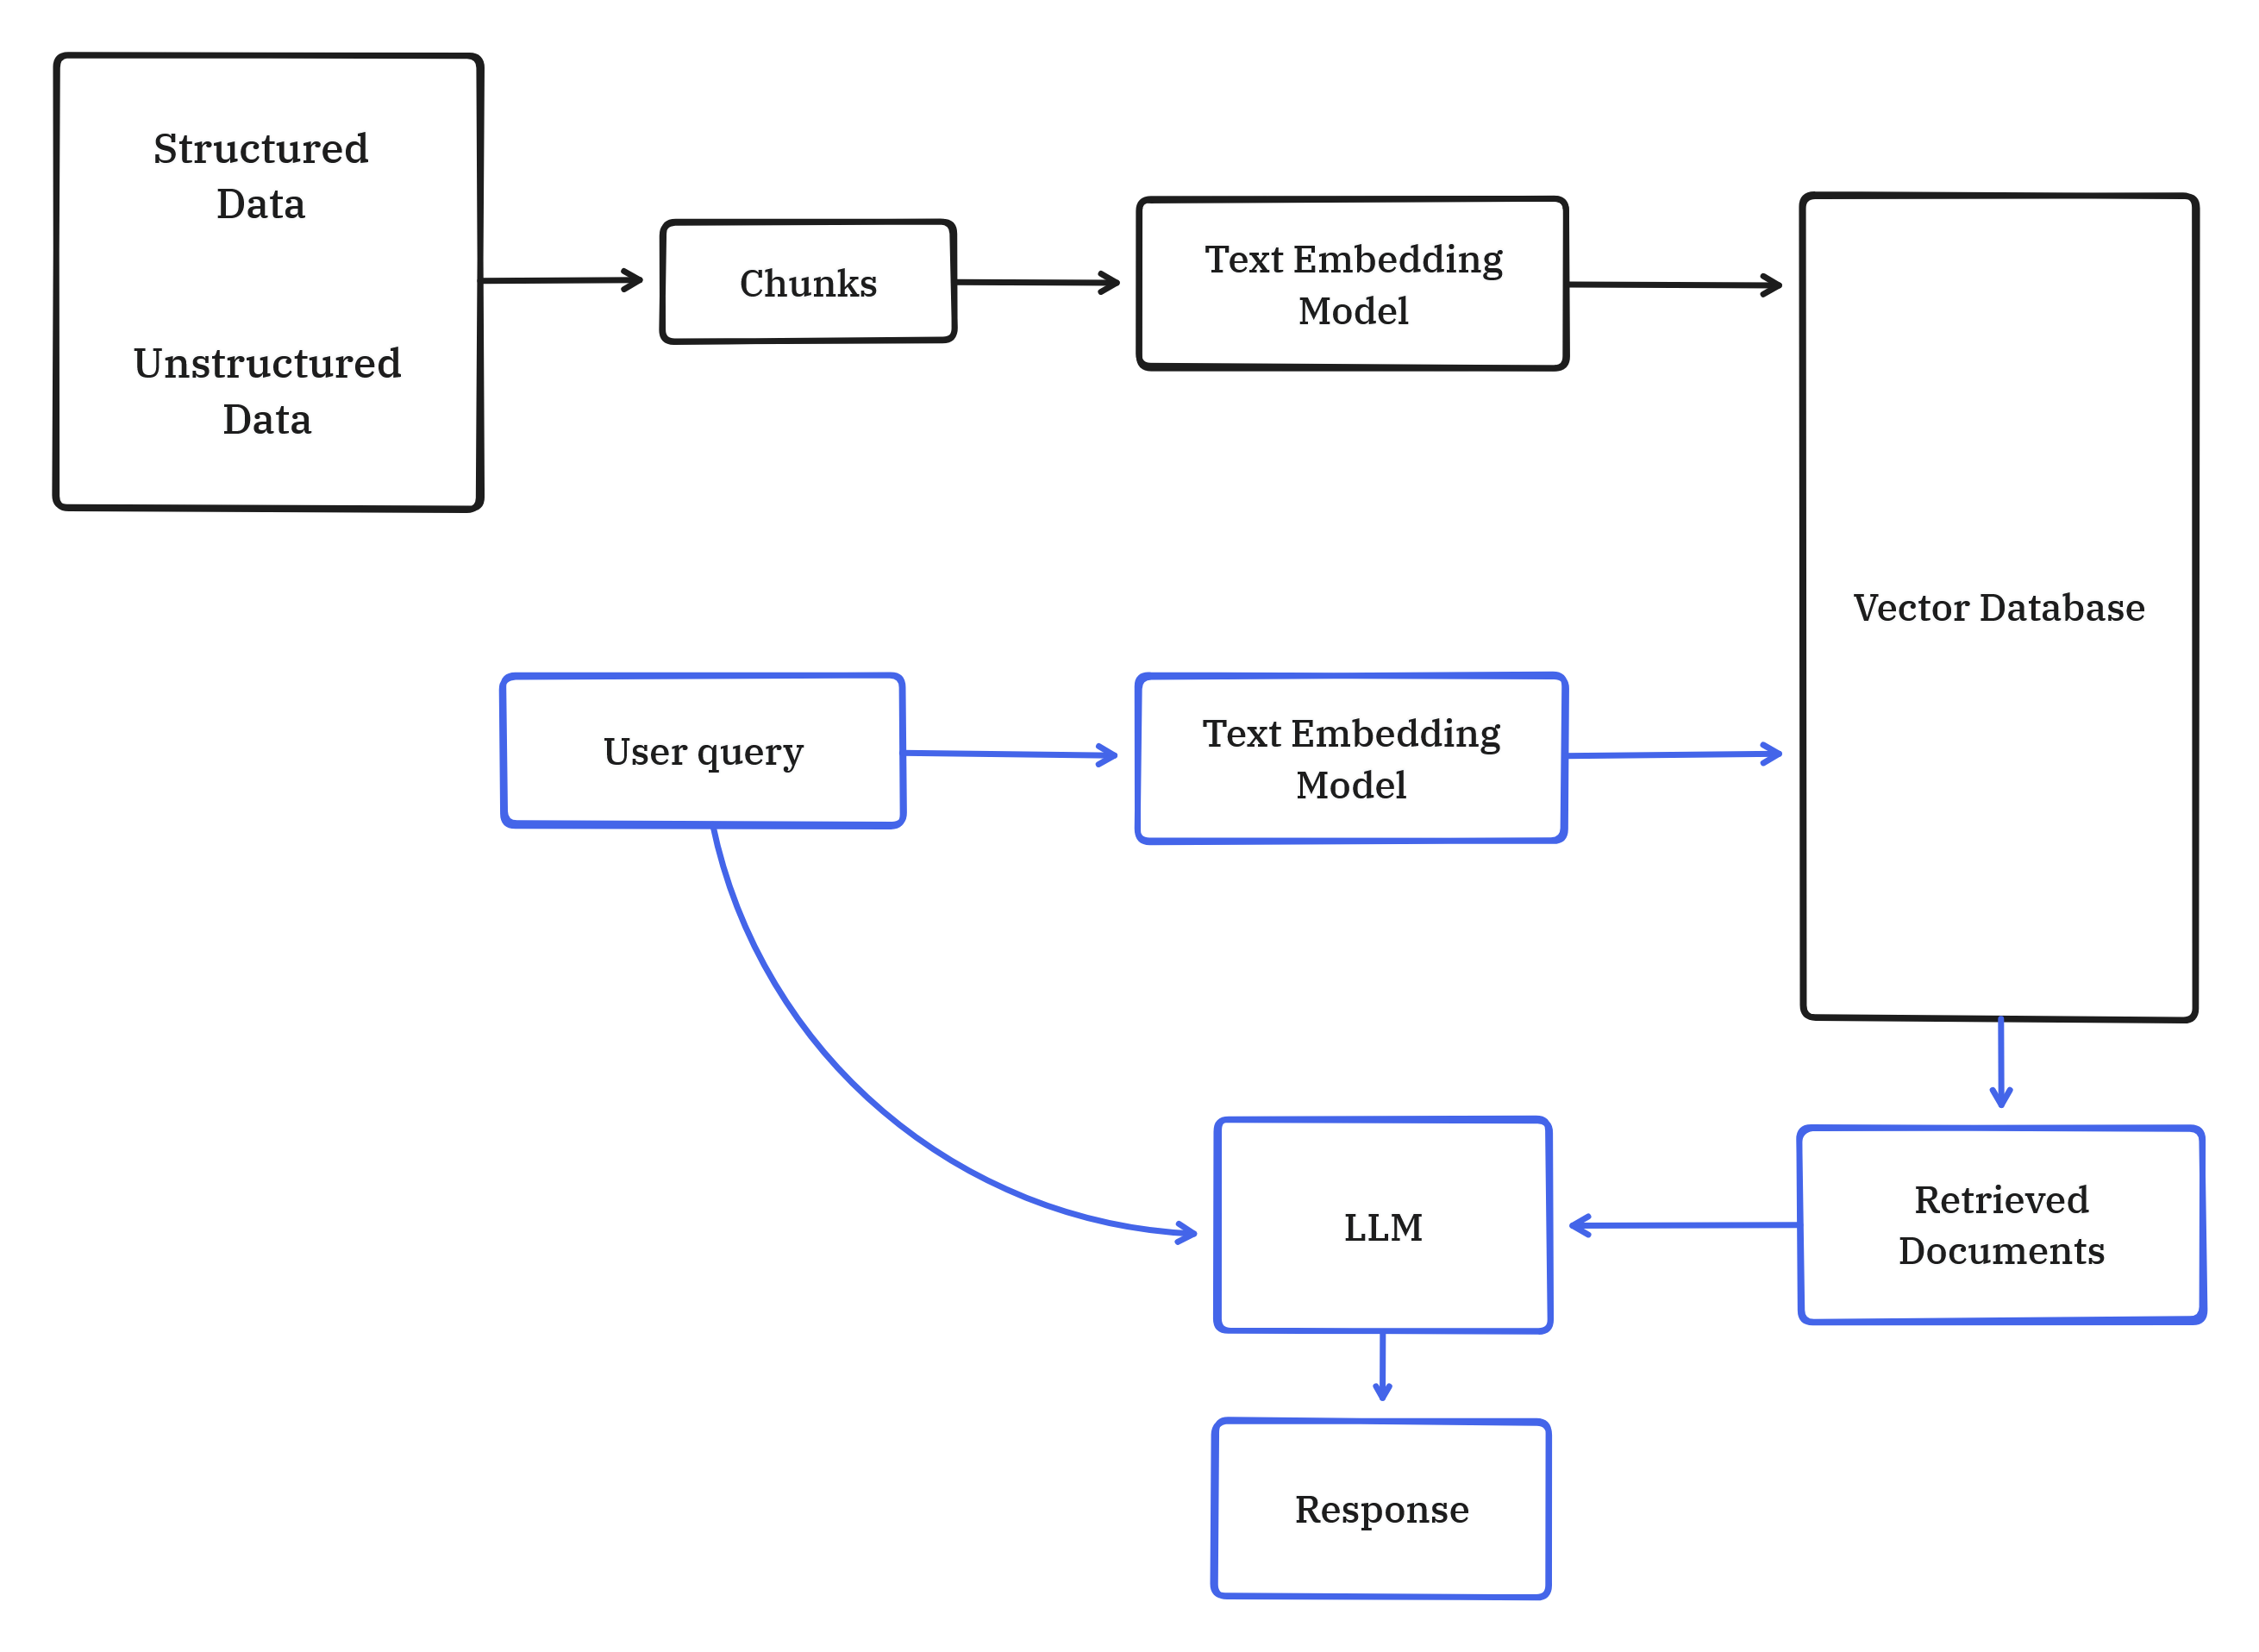
\includegraphics[width=\textwidth]{Conventional RAG example.png}
	\caption{Example of a Conventional RAG system}
	\centering
	\label{fig:RAGexample}
\end{figure}

RAG operates by retrieving relevant documents from an unstructured or structured vector database and providing them as context for response generation. To facilitate retrieval, documents are converted into vector representations using a text embedding model, which captures the semantic relations in text. When a query is presented to an LLM with a RAG system, the query undergoes the same text embedding process. The vectorized query is compared with the document vectors present in the database and those that have the highest similarity are returned to the LLM.

Through RAG, an LLM becomes able to generate highly accurate, domain-specific information rather than rely on its pre-trained knowledge, allowing for flexible applications in various fields.

One application of RAG in healthcare is in diagnostic assistance, where LLMs match patient symptoms with medical knowledge retrieved from external sources. This enables more informed diagnoses while reducing the cognitive load on physicians. Furthermore, LLMs may be able to detect subtle symptom correlations that clinicians might overlook, improving early disease detection \autocite{jin2024healthllmpersonalizedretrievalaugmenteddisease}.


Despite the benefits of RAG, it introduces vulnerabilities that must be addressed. RAG systems remain susceptible to prompt attacks much like LLMs are. They can also become poisoned, where the RAG corpus becomes corrupted through the insertion of adversarial attack passages.

In chapter \ref{literature} we discuss more about the vulnerabilities that RAG systems have.

\subsection{LLMs in Healthcare}

For Singapore in particular, LLMs have seen increased usage in healthcare. In 2013, Singapore's National University Health System (NUHS) launched its very own LLM, Russell-GPT, that was used for summarizing patient clinical notes, automating referral letter generation, as well as predict the healthcare journeys for patients \autocite{NUHS_2023}.

Singapore has also developed an LLM capable of understanding the local english dialect, Singlish, which has deployed in various settings, including clinics and emergency response systems, where it is used in transcribing emergency calls \autocite{Chia_2024}.

These developments showcase the growing reliance on LLMs in Singapore's healthcare ecosystem, highlighting their potential to improve the efficiency of its healthcare system. However, as LLMs become increasingly integrated into critical systems, it is essential to address the risks of their use - particularly when augmented with enhancements like RAG. RAG-powered LLMs remain vulnerable to adversarial attacks, risking the exposure of sensitive medical information. As such, ensuring that the security and privacy of LLM-based solutions remains a priority as they continue to evolve.

\chapter{Literature Review} \label {literature}
\section{Background}


\subsection{Exploitation of RAG Systems}
Studies (\cite{tan2024gluepizzaeatrocks}; \cite{zeng2024goodbadexploringprivacy}; \cite{xue2024badragidentifyingvulnerabilitiesretrieval}) have shown that RAG systems are susceptible to well-crafted prompt attacks during the retrieval stage.

By using targeted as well as untargeted attacks \autocite{zeng2024goodbadexploringprivacy}, a malicious attacker is able to retrieve personally identifiable information (PII), such as phone numbers and addresses, from a RAG's corpus.


\autocite{tan2024gluepizzaeatrocks} and \autocite{xue2024badragidentifyingvulnerabilitiesretrieval} showcase the ability to affect an LLMs output by inserting specially crafted adversarial passages into its RAG corpus.

This typically affects LLMs that make use of real-time context databases, such as a search engine, which allows an attacker to insert malicious documents into the context database.

\subsection{Large Language Model (LLM) Safeguards}
The widespread usage of LLMs necessitates the development of safeguards to prevent ethical misuse and abuse.
These safeguards are often times complex, varying based on application requirements.
\autocite{dong2024buildingguardrailslargelanguage} discusses the different components involved in implementing guard rails for LLMs and touches on some of the currently deployed solutions available.
In general, safeguards are designed to prevent the LLMs from generating unintended output.
This unintended output can be generated in numerous ways, most notably through ``hallucinations'' as well as targeted prompt attacks known as ``jailbreaking''.

\chapter{Methodology} \label{methodology}
\section{Description of Pipeline}
Based on research into RAG vulnerabilities, there is a clear lack of security measures designed to preserve the privacy of a RAG corpus. This is especially important in fields like healthcare.
As demonstrated in \autocite{zeng2024goodbadexploringprivacy}, private information can be easily extracted by determined attackers through simple prompt injections.
Given that RAG relies on a set of documents as context and its vulnerabilities to RAG, we believe that generating a synthetic document separate from the corpus is sufficient to mitigate most issues.

\section{System Design}
As mentioned, the solution explored in this project consists of an agent-based document synthesis pipeline aimed at preventing raw LLM access to sensitive data.

For all intents and purposes, the pipeline operates in a similar fashion to typical RAG. Upon receiving a query, it fetches document from the RAG corpus then uses the retrieved documents as context in generating a response. However, we include an intermediary step between the information retrieval and inference steps.

Once the documents are retrieved, a  secondary LLM extracts only the necessary information from the documents retrieved. For instance, we may retrieve a medical record consisting of different medical readings for a query about a patient's blood pressure readings. In this example, we aim for the LLM to extract only the blood pressure readings from this document.

With the information retrieved, we use an agent-based approach to modify the information. In order to further distance the information from the original record, we apply the following steps.

Firstly, we remove any PII that may appear in the information. We consider the following as PII: names, ages, contact number and address. The LLM will remove, or replace with pseudonyms, any appearance of PII.

Secondly, we manipulate the data that appears in the information to generalise the record. Numbers are rounded, and converted to ranges if multiple readings of the same type occur.

Finally, to ensure that the LLM treats the synthesized information as relevant context, we modify the original query based on the synthetic information. It should be able to generate the same output as a model operating solely on RAG.

Once it has gone through this step, we pass the synthesized query and information to the primary LLM to generate a response.

Refer to figure \ref{fig:SynthLLMRAG} for a visualization of the system design.

\begin{figure}
	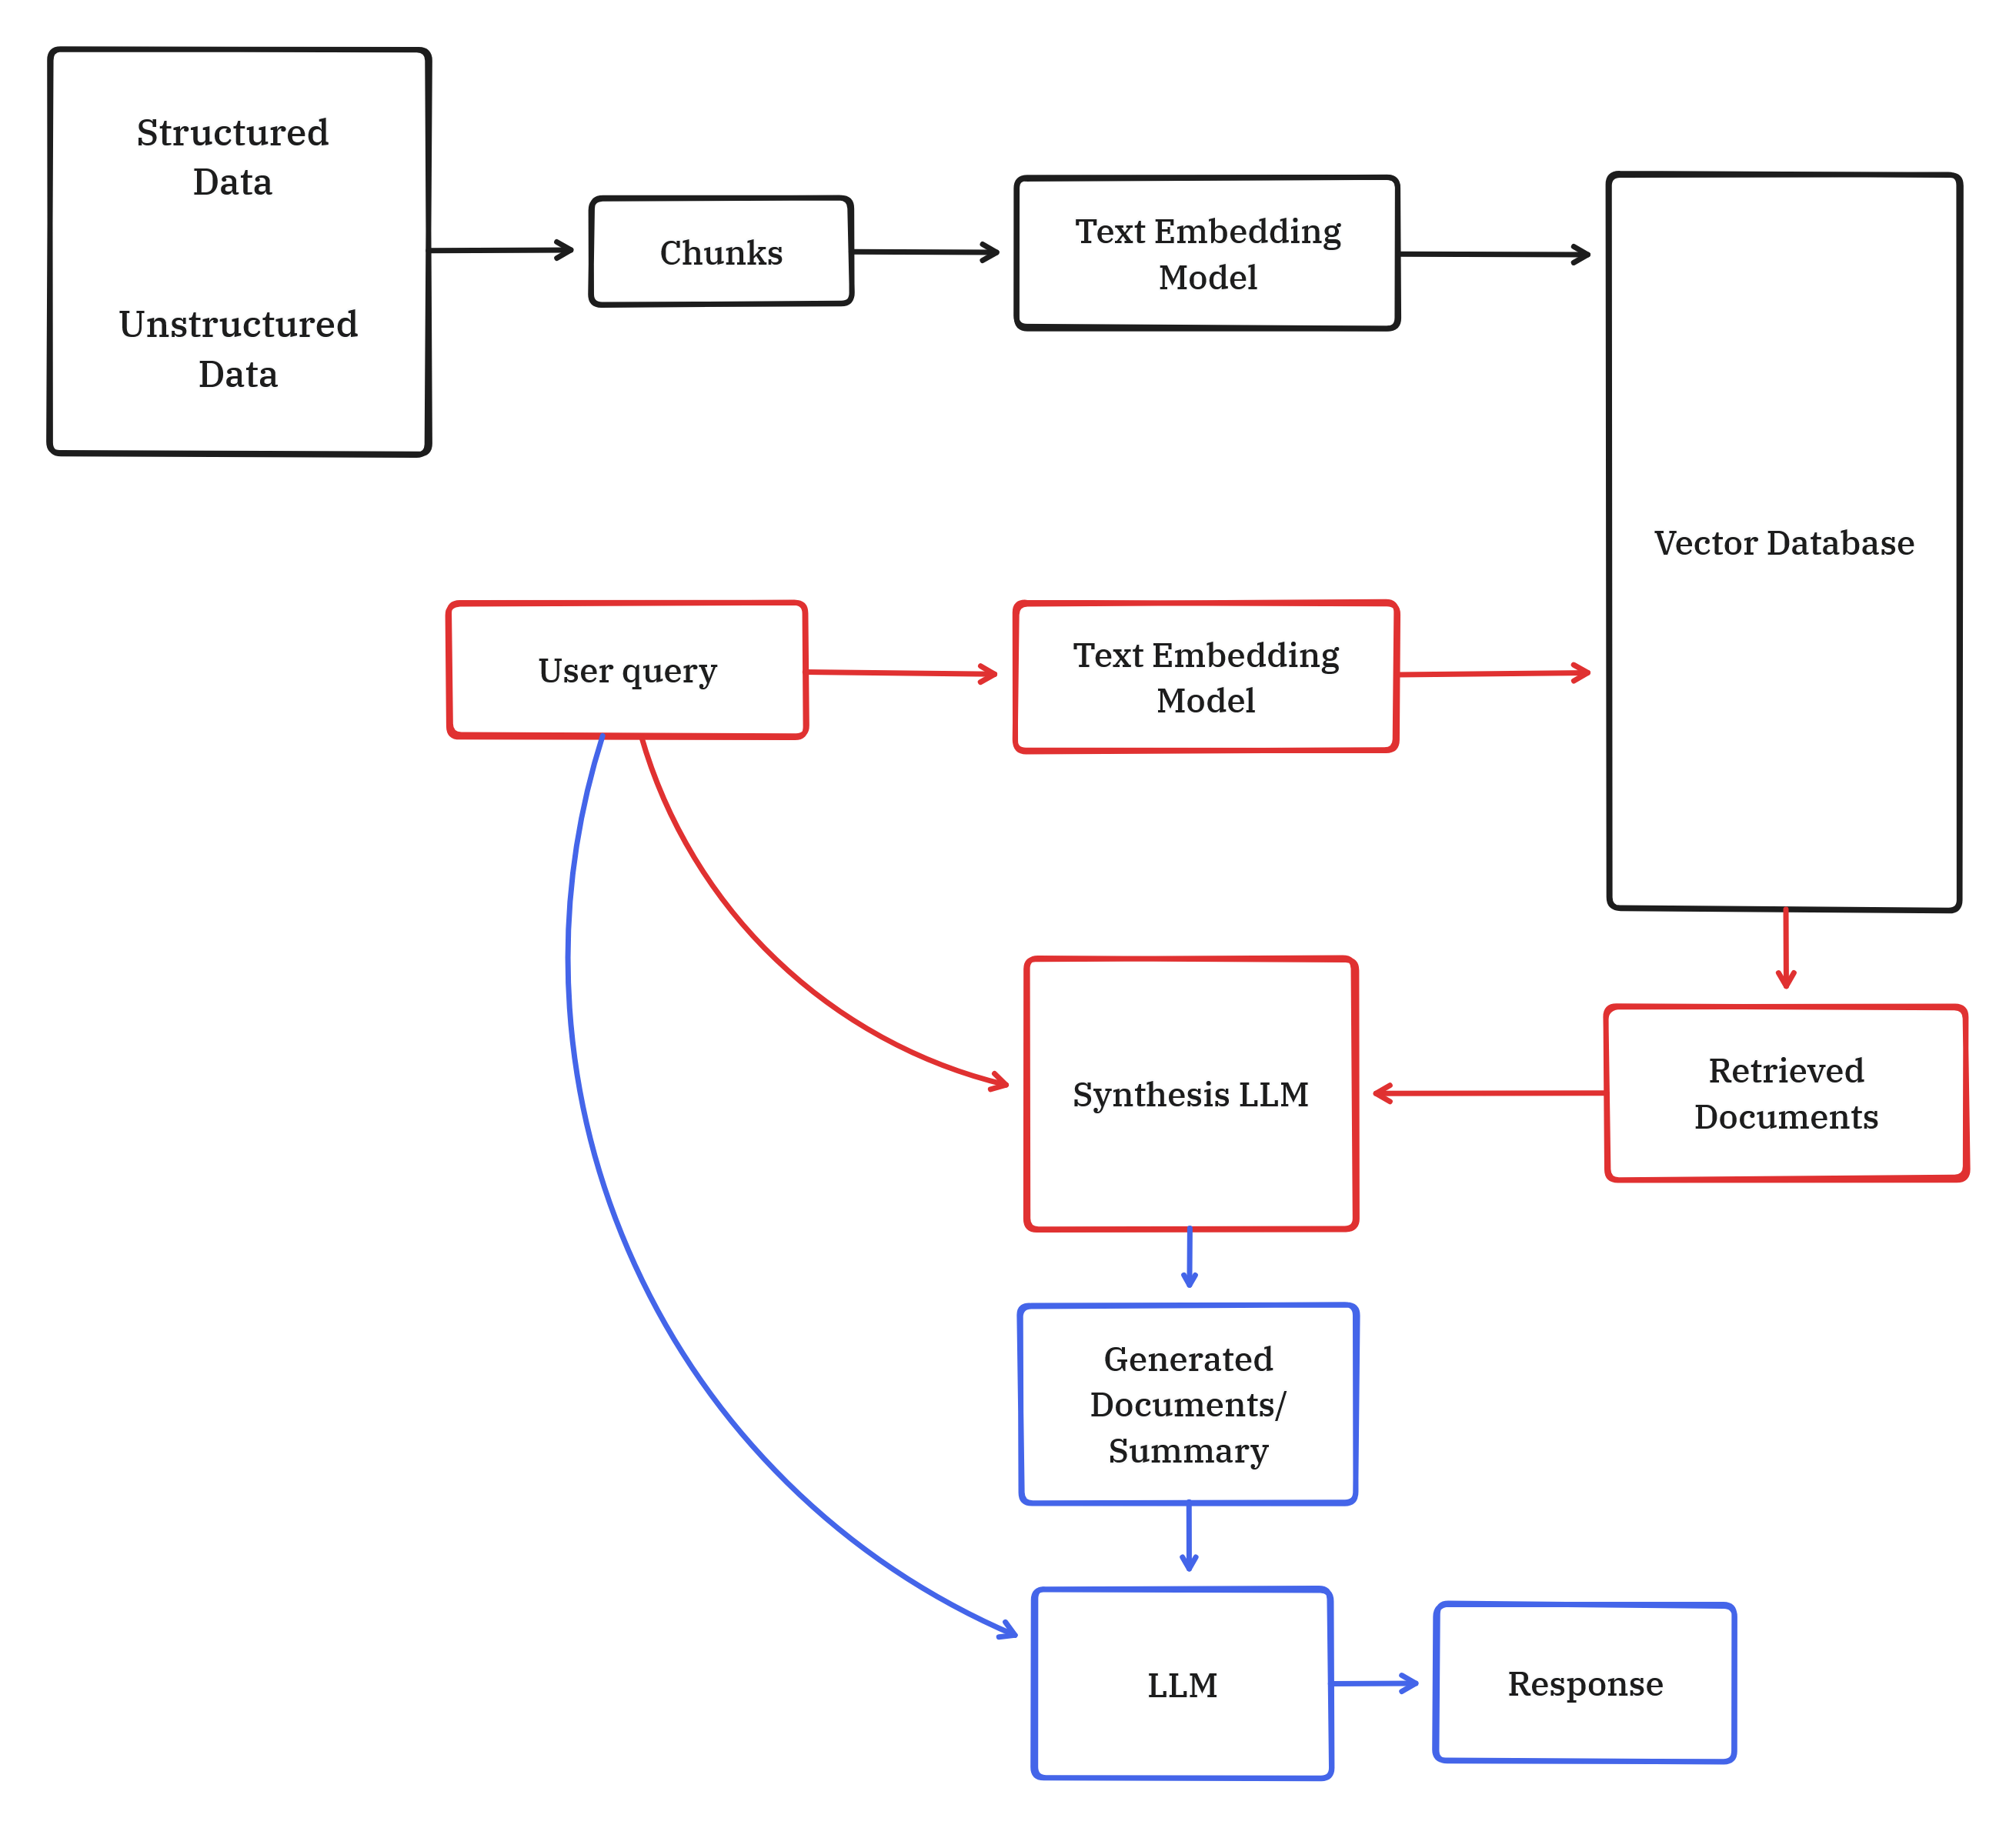
\includegraphics[width=\textwidth]{Synthesis LLM RAG example.png}
	\caption{System Design}
	\centering
	\label{fig:SynthLLMRAG}
\end{figure}

\section{Building the RAG Corpus}
RAG systems can make use of either structured or unstructured data, however in healthcare, data is usually structured.
In order to mimic real healthcare settings, we determined it was necessary to make use of data that was designed for real-world settings.
For our case, we will be making use of a synthetic Fast Healthcare Interoperability Resources (FHIR) dataset, generated and distributed by Synthea \autocite{Synthea2024}.

FHIR is a structured healthcare standard that defines how healthcare information can be shared between different systems regardless of how they are stored.
Individual FHIR patient records are stored in what is known as resources and each resource type represents specific information. A Patient resource would include the patient's name, date of birth, address, etc. Each resource type is specific to its use case.

FHIR records can appear in different file formats, JSON, XML, or RDF. For simpler parsing and handling, we will be making use of JSON FHIR files to build our RAG corpus.

We make use of the open-source library \textbf{Llamaindex} \autocite{Liu_LlamaIndex_2022} for abstractions when building the pipeline, as well as creating the database.

\subsection{FHIR Preprocessing}

First, we consider the type of data we wish to embed. JSON files are designed for programmatic use, meaning that they contain many identifying and delimiting tokens. If we were to convert the file in its entirety into its vector representation, it will result in detail being lost due to the repeated embedding of same key-value token pairs. Therefore, we first have to carry out flattening of the FHIR record.

Flattening the FHIR involves two things. First, we must determine what type of information we wish to extract. For this project, we are only working with information from the Patient resource, as well as the Observation, Procedure, Condition, Allergy and MedicationRequest resources. While initially the Encounter resource was used, we decided that it did not add any type of substantial information apart from the reason of the encounter as well as the location where it took place. Secondly, we have to convert the selected information into basic sentences. This is done by recursively un-nesting the FHIR resource with the information we specified. Refer to figure \ref{fig:FHIRtoSentence} for an example.

\begin{figure}
	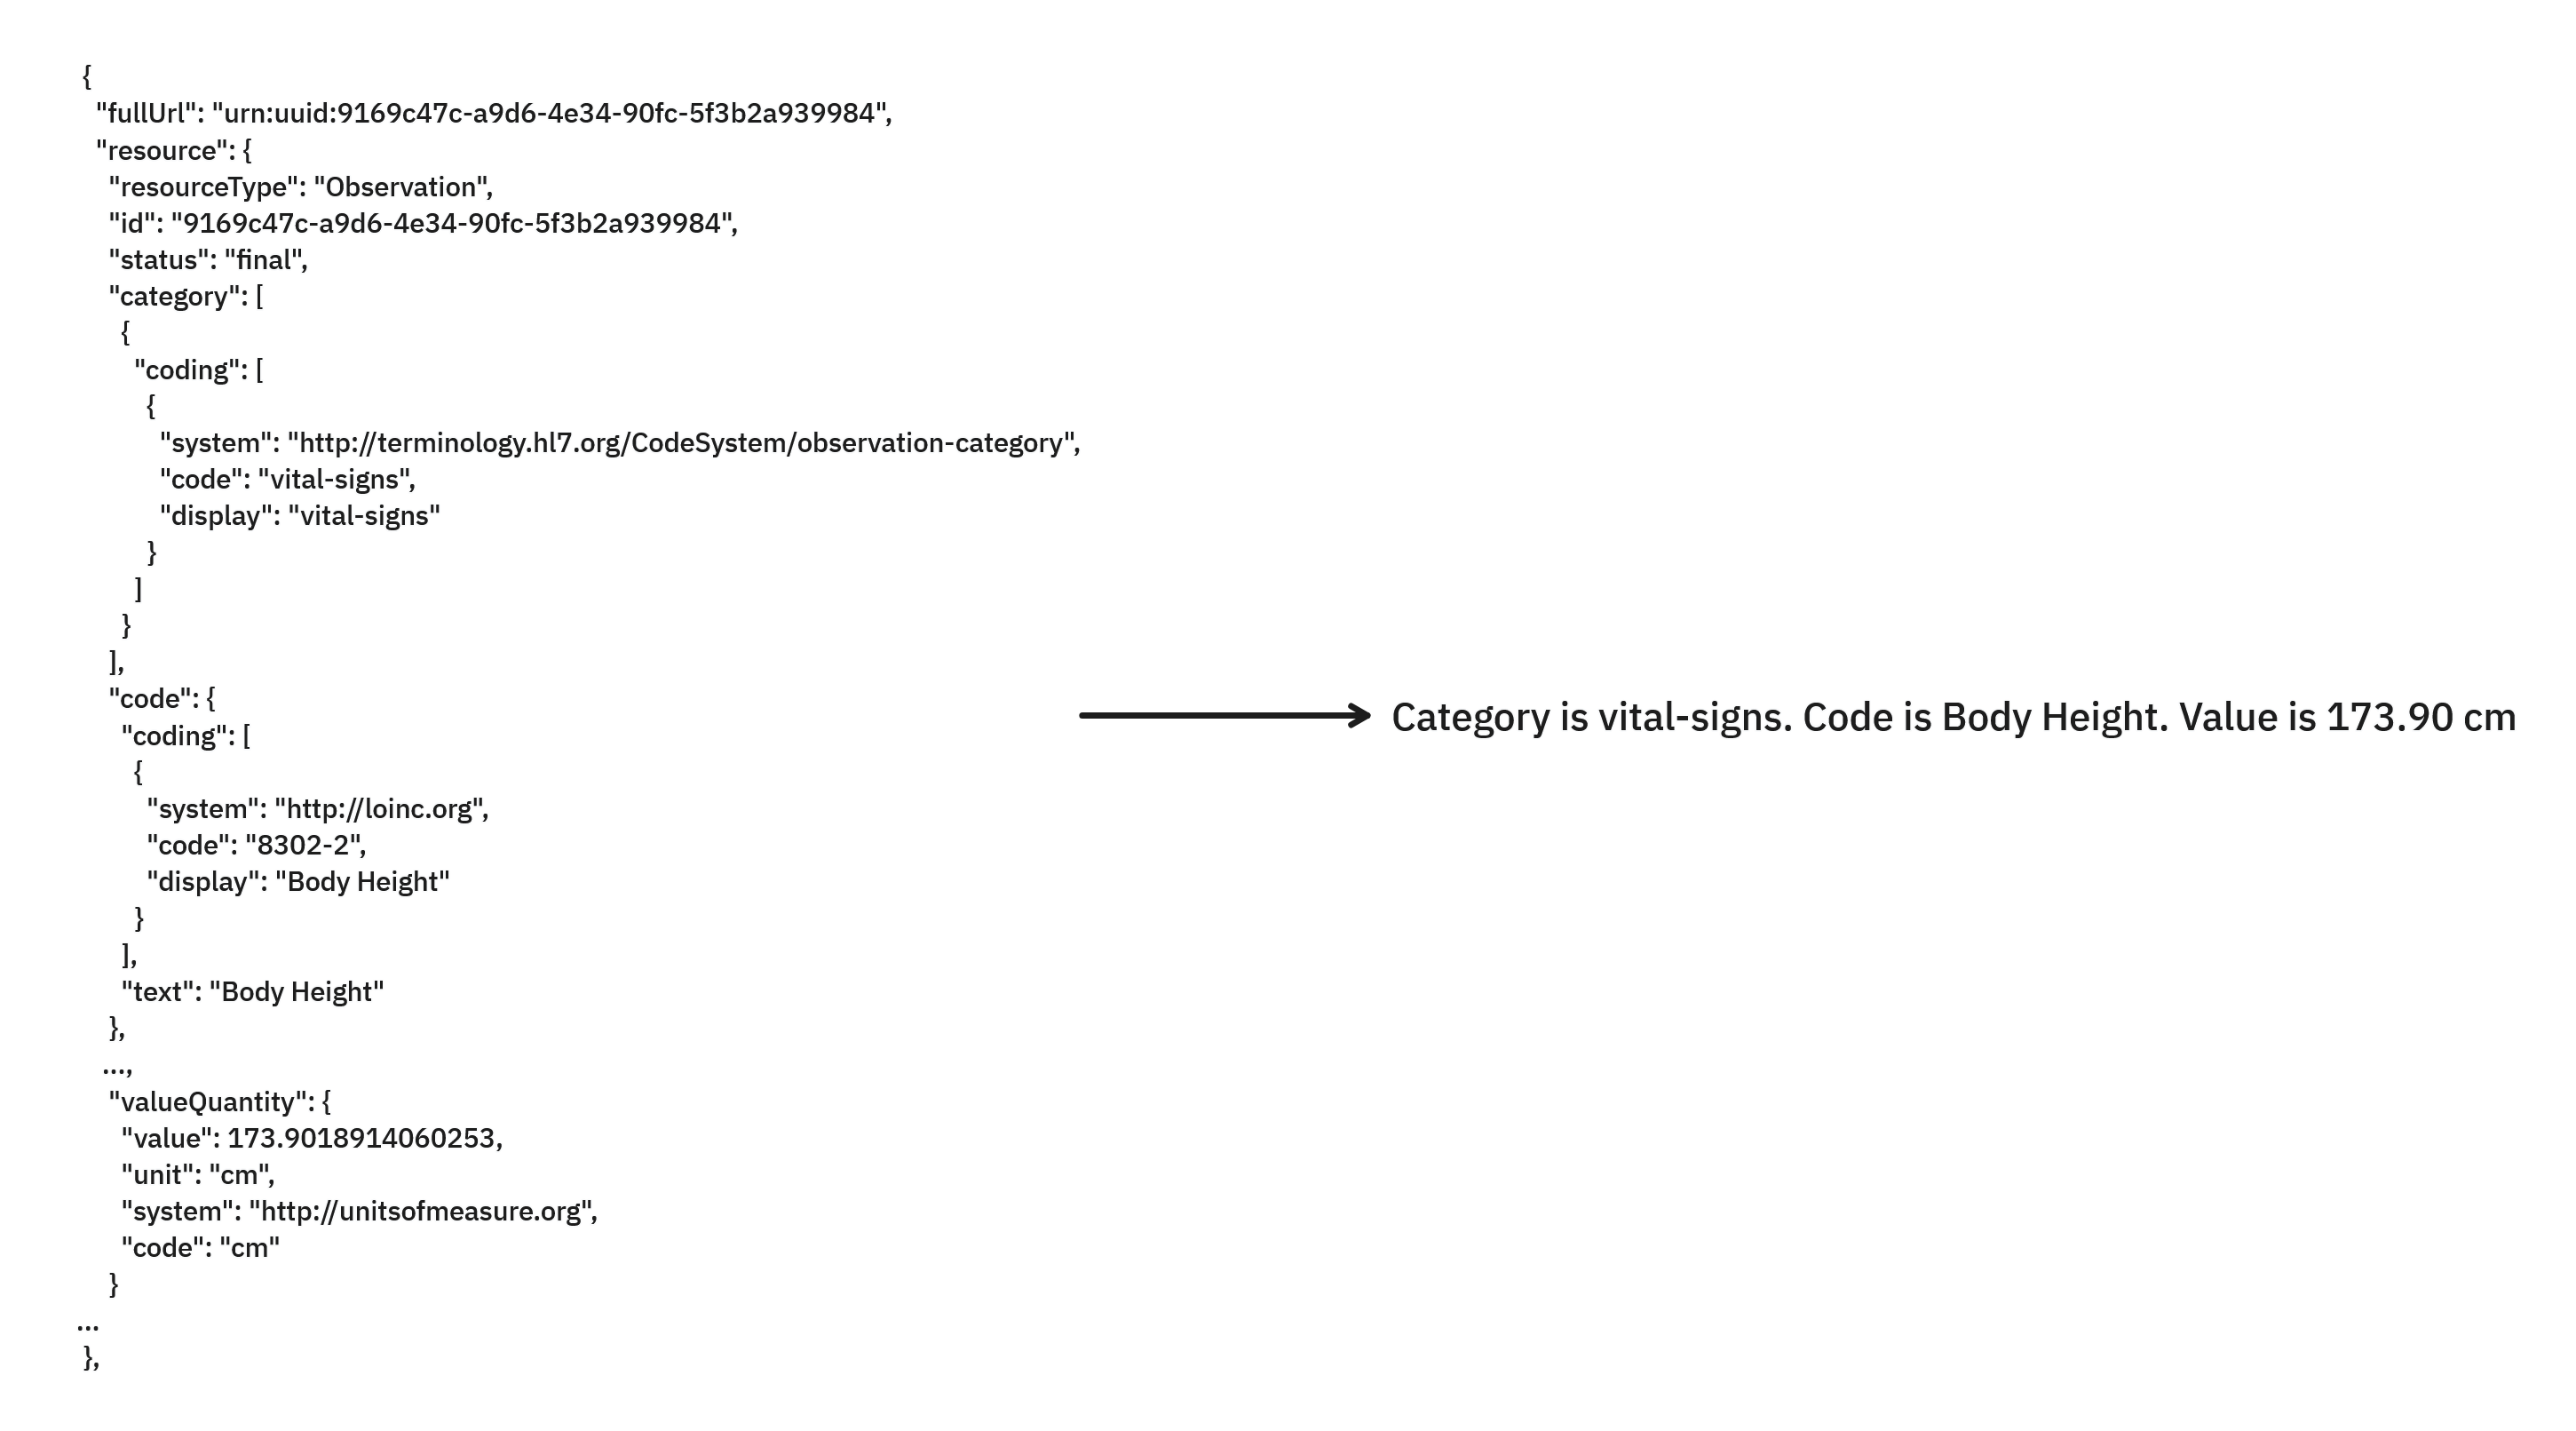
\includegraphics[width=\textwidth]{Converting FHIR to sentence.png}
	\caption{FHIR to sentence}
	\centering
	\label{fig:FHIRtoSentence}
\end{figure}

Processing the FHIR record, we group the information extracted from the Observation and Procedure resources by date. Afterwards, we collate the conditions, allergies, as well as the medications that has been assigned to the patient previously.

Using the archive officially distributed by \textbf{Synthea}, which contains 101 synthetic patients, we end up with a total of \textbf{5931} files. Figure \ref{fig:FileDistribution} shows the file distribution across patients. As we can see, there is a significant number of synthetic patients with over 100 files.

\begin{figure}[h]
	\centering
	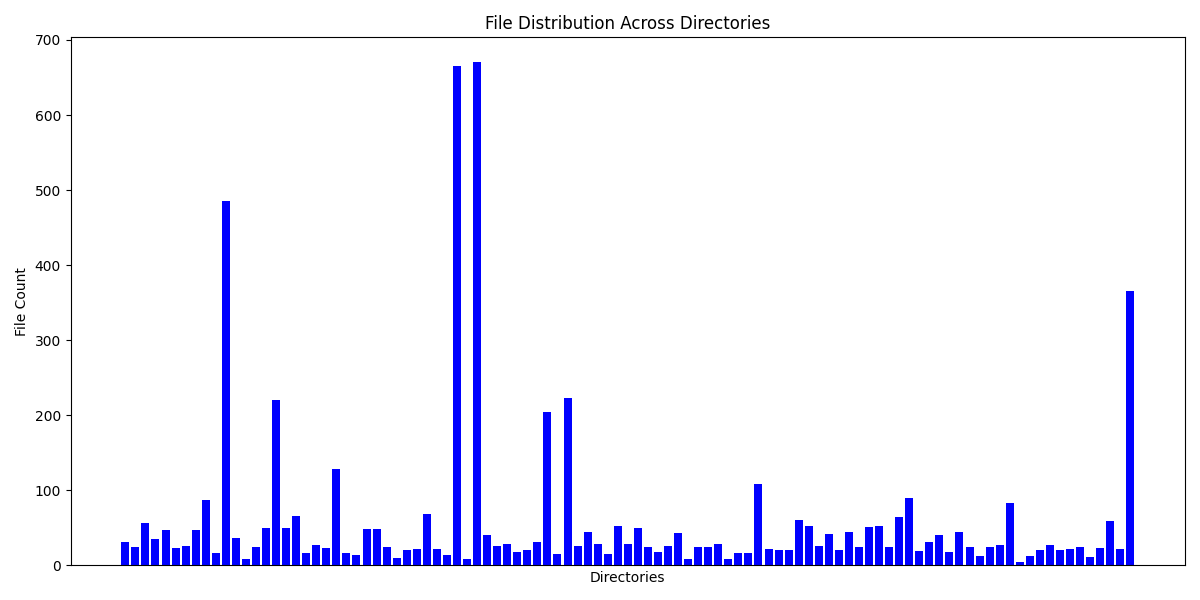
\includegraphics[width=\linewidth]{file_distribution.png}
	\caption{File Distribution}
	\label{fig:FileDistribution}
\end{figure}

Over concerns about whether this will affect the retrieval results, we decided to remove any outliers that appear. How do we define outliers? By inspection we see that, on average, synthetic patients have around 40 to 60 files per patient, with few approaching 80 to 90 files.
Removing them, we end up with the following new distribution as seen in figure \ref{fig:FileDistributionAfter}. As we can see, we end up with a more reasonable distribution.

\begin{figure}[h]
	\centering
	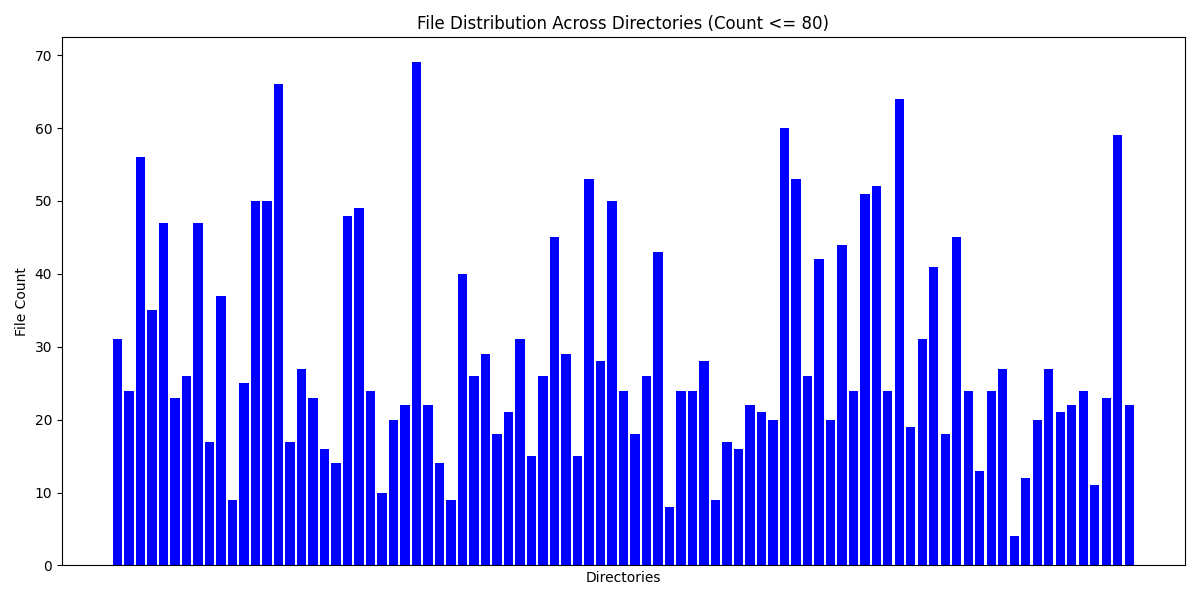
\includegraphics[width=\linewidth]{file_distribution_trimmed.png}
	\caption{New File Distribution}
	\label{fig:FileDistributionAfter}
\end{figure}

Each of these documents are stored in separate files, marked by the patient's name followed by the date of the encounter to facilitate the document embedding process.

\subsection{Generating Embeddings and Keywords}

With the documents processed, we move on to embedding the documents. Vector embedding is the process of converting values to their vector equivalents, which are essentially a list of numbers representing our value.
By doing this, we can approximate the semantic similarity between objects through their proximity within the vector space. This makes it useful for RAG applications where semantic searches are common.

Before generating the vector embeddings from the documents, we have to consider which embedding model to use. Given that we are working with text, we looked towards text embedding models. Here the differences between models vary in size and performance. For this project we make use of open-source model \textbf{bge-base-en-v1.5} to generate the vector embeddings for the documents.

Each document is passed to the transformer model where it outputs the corresponding vector representation, then stored within the database. There are a number of different possible databases designed for vector embeddings, however, in this project we make use of the \textbf{Postgresql} database as well as the \textbf{pgvector} extension in order to enable vector storage.

In the process of generating the embeddings, we also generate a list of keywords that appear in the text document, storing them in separate indexes. This is to facilitate both keyword and semantic searches in the RAG system.

The overall process of the embedding generation is outlined in figure \ref{fig:EmbeddingsDatabase}.

\begin{figure}
	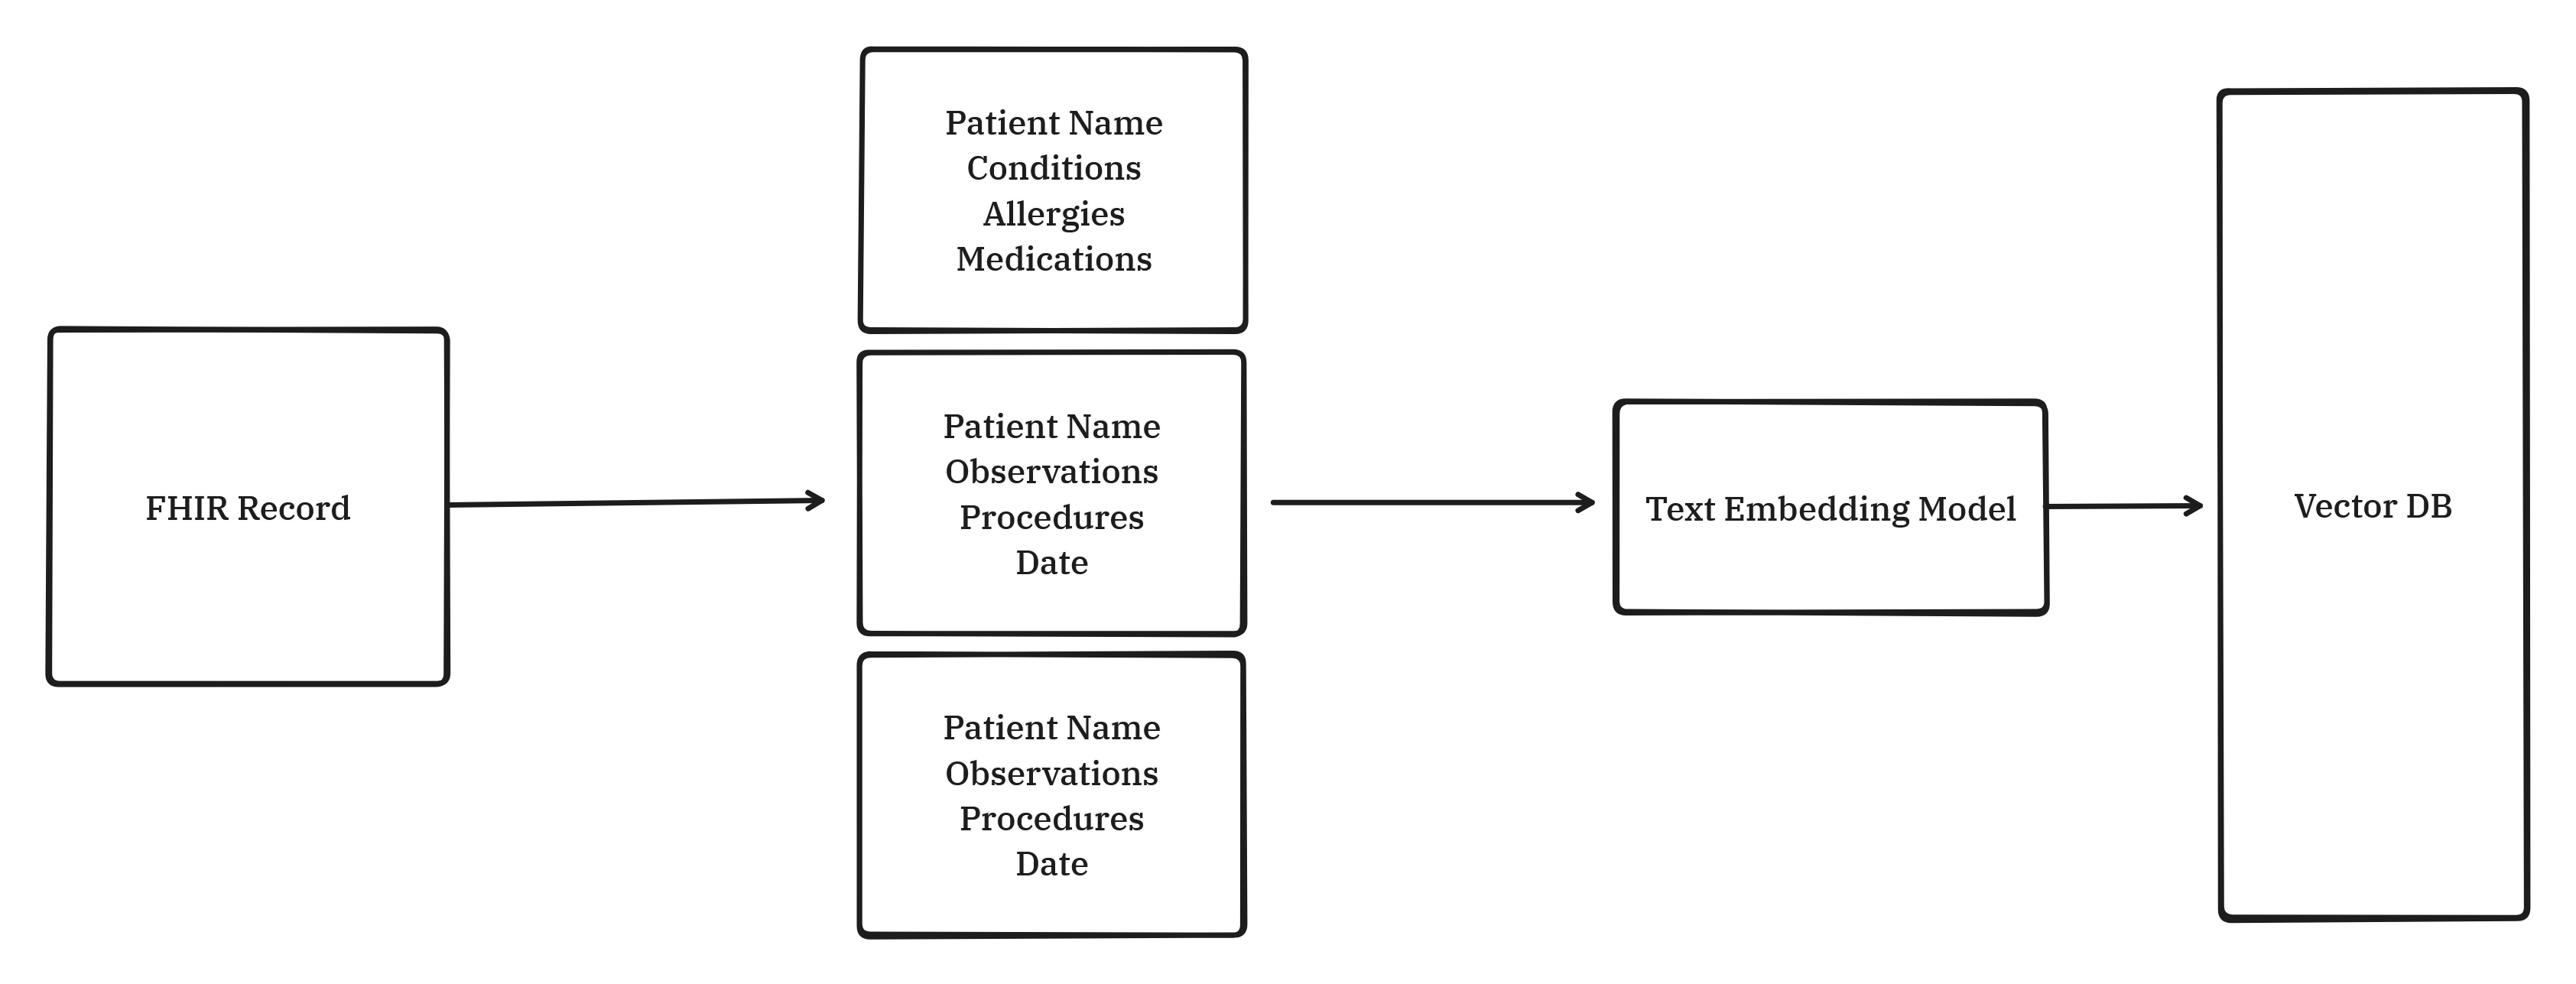
\includegraphics[width=\textwidth]{Store embeddings in DB.png}
	\caption{Embeddings to Database}
	\centering
	\label{fig:EmbeddingsDatabase}
\end{figure}

\subsubsection{Generating Questions}

After the process of creating the corpus, we also generate a single question based on the contents of each file. This is to test the accuracy of the RAG retrieval later.

Each file is passed to a LLM with the following prompt: \textit{"Generate a single question about the following text. Avoid general queries such as marriage status, death, age, contact, address. Text: $\{text\}$"}, and once the questions have been processed we store them in a JSON file for use later.

In general each question contains a piece of information contained within the text file, as well as the date associated.
\section{Large Language Model Choice}

With our RAG corpus processed and populated, we now look towards selecting the LLM to serve as the basis of our agents.
Not all LLMs are made equal, and a general convention is that the larger, the more sophisticated its response.
The intuitive choice is to make use of a well-established third-party LLM like OpenAI's ChatGPT, however, this is not acceptable due to the fact that it is a closed, proprietary model. In a field like healthcare, where private and sensitive information will be distributed, this is non-negotiable since it cannot be guaranteed that the data shared with ChatGPT will not be used for training or other purposes.

Given this reasoning, we look towards open-source LLMs. For our requirements, the LLM has to be able to make use of tools. Tools are functions that the LLM can call to perform a specific action. For example, it could call a function to add or subtract two numbers. In this project, functions are used to allow the LLM to perform searches on our RAG corpus.

There are a few notable LLMs that can make use of tools, such as Alibaba's reasoning model \textbf{QwQ}, Meta's \textbf{Llama3}, and Mistral AI's \textbf{Mistral}. In this project we decided to make use of Alibaba's \textbf{Qwen-2.5-32B}. It is a decent baseline model that performs adequately in all aspects, and we do not require the capabilities of a reasoning model like \textbf{QwQ}, as that will add to the total inference time.

\section{Agent Workflow Design}

Now that we have decided on the model to use, we move to designing the agents that will be involved in the workflow.

The document synthesis pipeline consists of three agents, each with their respective prompts.
There is the Synthesis Agent, which is in charge of transforming the information that is retrieved. The Search Agent is in charge of carrying out the necessary semantic searches on the database using the input query. Finally, the Review Agent is in charge of checking the synthesized information generated by the Synthesis Agent.

The prompts for each agent are available in appendix \ref{agent prompts}.

Figure \ref{fig:AgentInteraction} outlines the flow of interactions between the different agents.

\begin{figure}
	\centering
	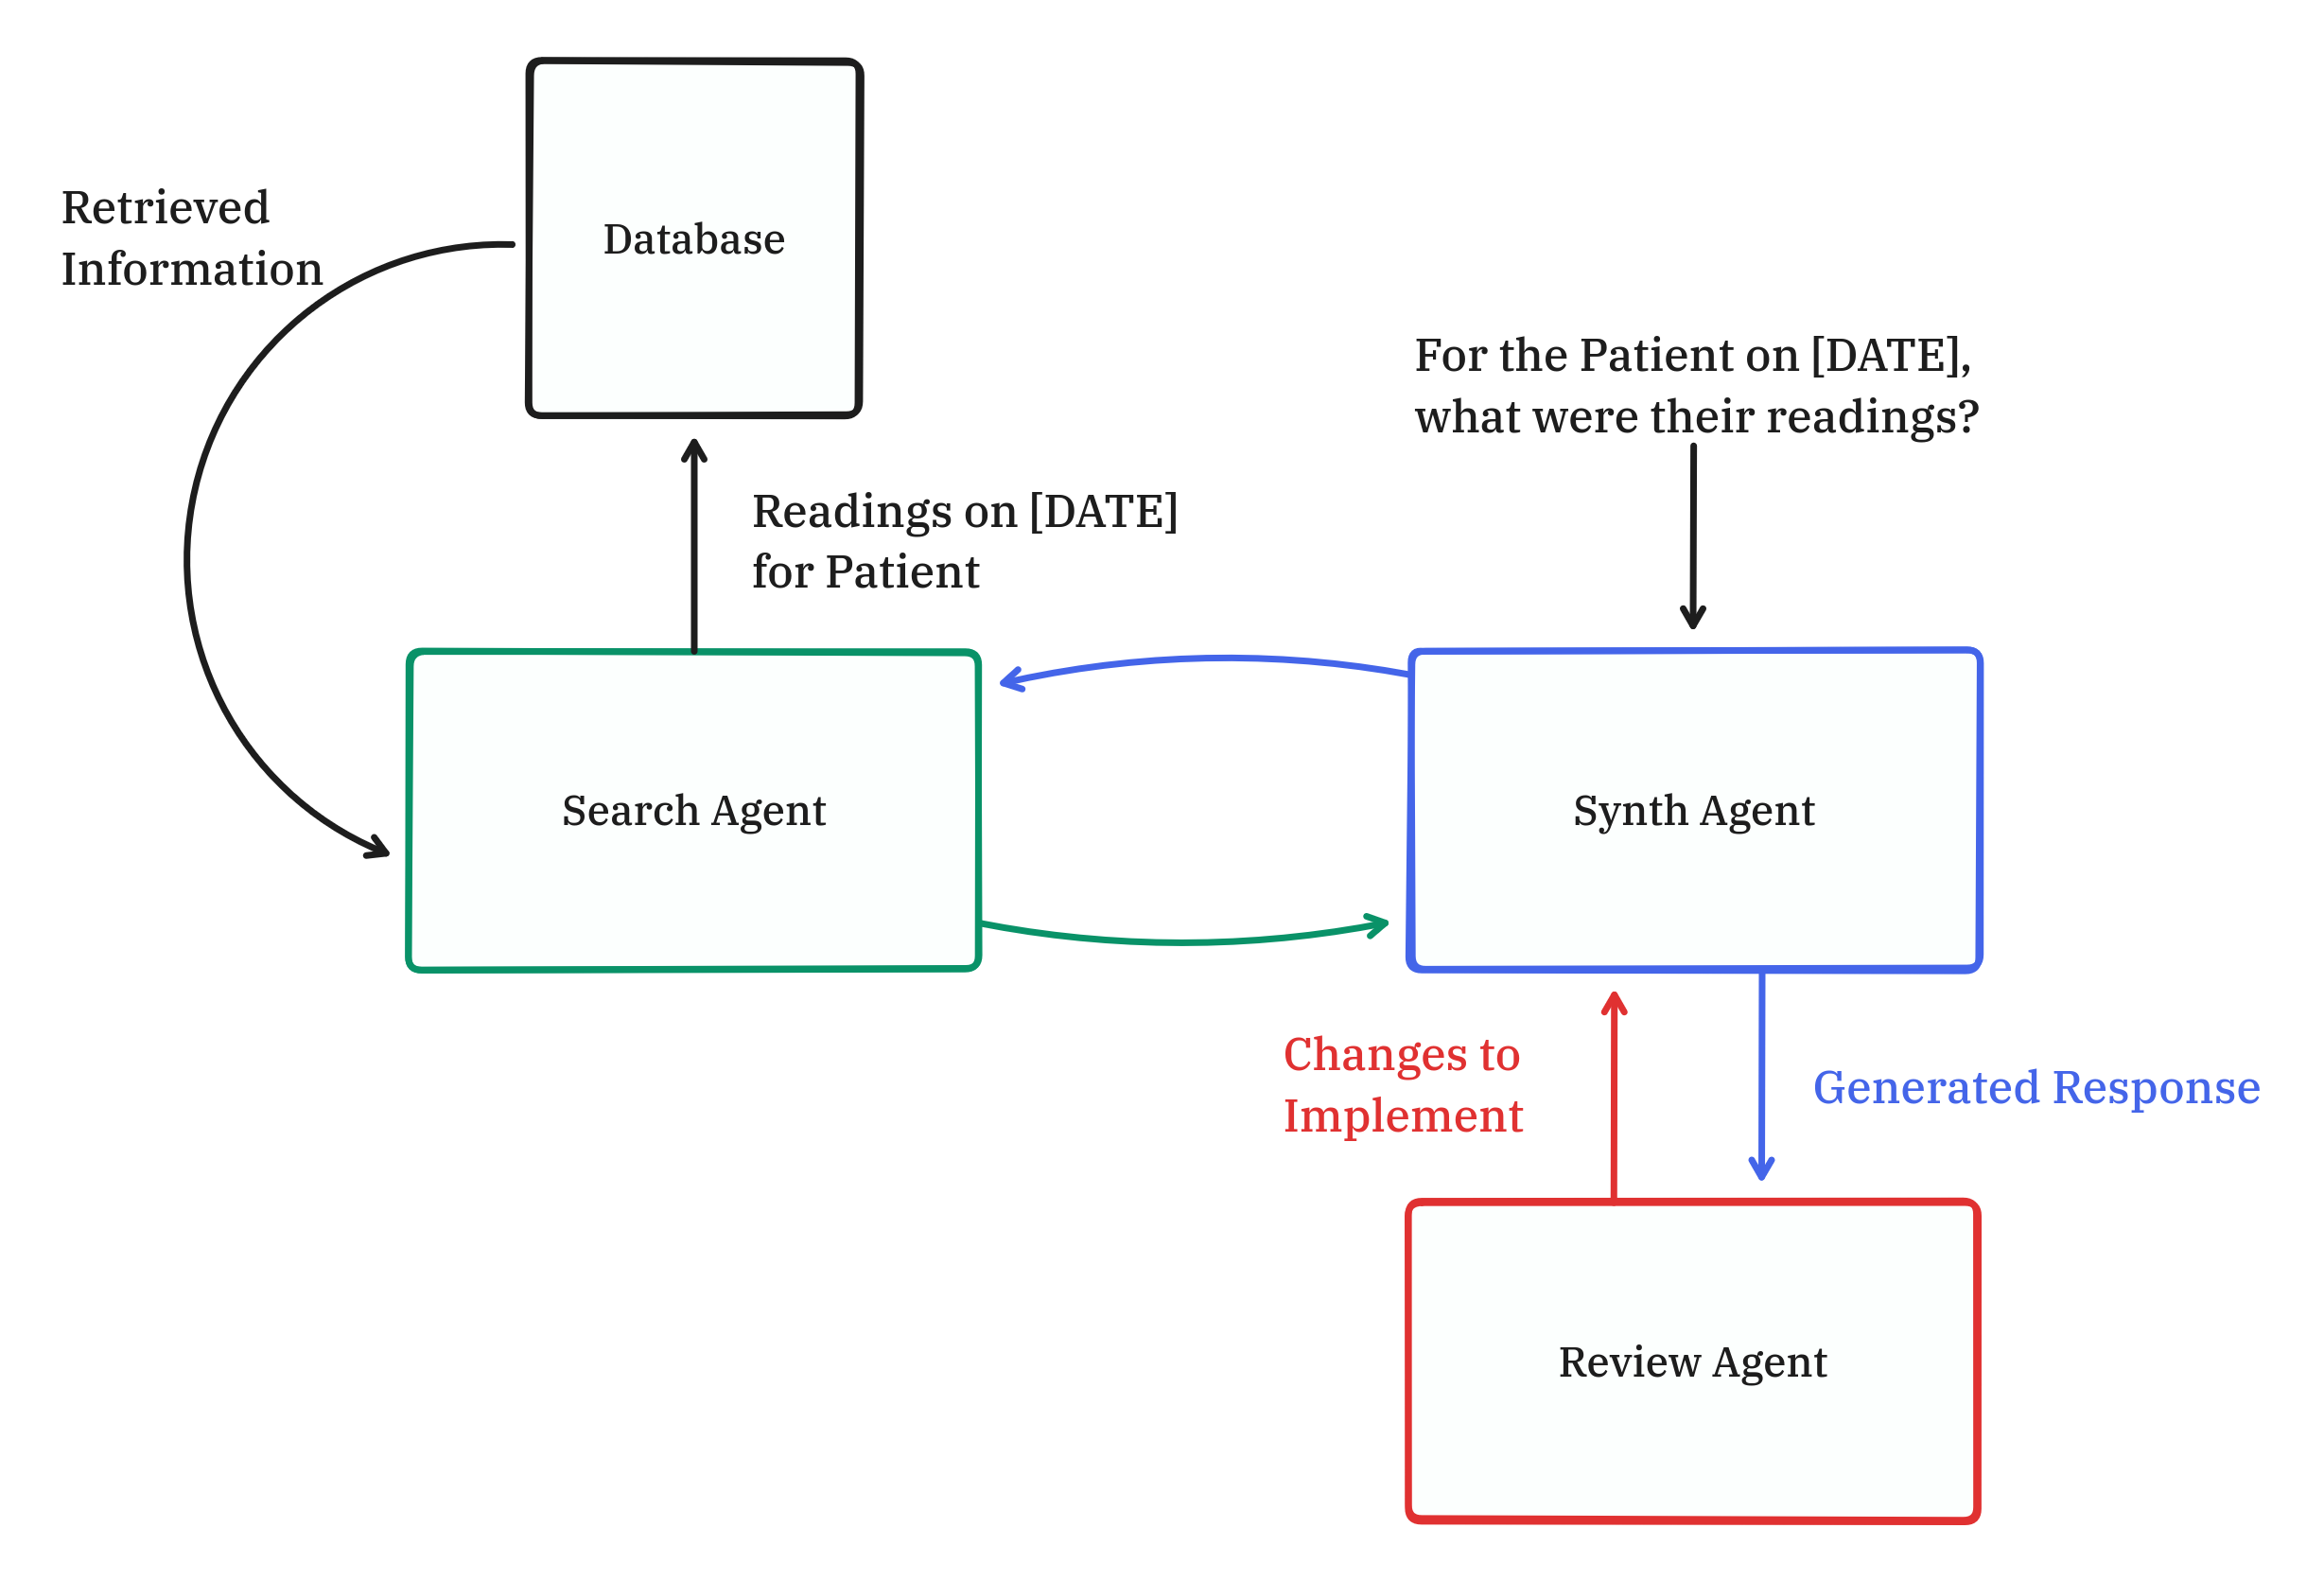
\includegraphics[width=\textwidth]{agent-workflow.png}
	\caption{Agent Interaction Flow}
	\label{fig:AgentInteraction}
\end{figure}

Upon receiving an input query, the Synthesis Agent passes off control to the Search Agent, which determines what kind of searches need to be run.

There are two ways the Search Agent can carry out searches. First, it can carry out a semantic search using information from the query. Secondly, it can check for patients that have been diagnosed with a specific condition. The logic behind this is to enable the Search Agent to carry out general queries, such as searching for medications given to patients diagnosed with the same condition.

Finally, once the necessary information has been consolidated, we return it to the Synthesis Agent.

The Synthesis Agent is in charge of transforming the information received. The main aspects that it changes is that it replaces names with pseudonyms, as well as attempts to remove all occurrence of PII within the retrieved information. Finally, it rounds off any numerical values that appear, and attempts to consolidate them into a range.

Using the newly synthesized information, it generates a new query in order to ensure that the LLM notices the relation between the synthesized context and query. The synthetic query may or may not differ from the original query, depending on the type of information retrieved, however the model should not produce a response that is too different from the baseline response.

The Review Agent's purpose is to ensure that the Synthesis Agent's response adheres to the guidelines set. It has been prompted similarly to the Synthesis Agent, however its main purpose is simply to point out any errors in the Synthesis Agent's response and allow for correction.

At the end of it, we will have a segment of text synthesized from the original documents that does not contain PII, with only the information that is needed to answer the input query.
\section{Agent Functions}

With the workflow outlined, we move into designing functions for each agent to call.

\subsection{RAG Worflow}


The retrieval method varies based on the type of information stored. In this project, we make use of semantic searches as well as keyword searches in our RAG system.

The semantic searches facilitate the retrieval of queries related to medical readings. This could be blood pressure, glucose, etc.

The keyword searches are targeted at looking up patients diagnosed with a specific condition. This is to facilitate two step searches. For example, an input query might ask \textit{"What medications are diabetes patients on?"}
If the agent only has access to semantic searches, it will not have enough information to answer the query unless we adjust it with a high \textit{k} value, but that does not guarantee that the nodes retrieved will be correct, because the search query will also be adjusted by the agent.

The process of semantic retrieval involves converting the input query into its vector equivalent in order to compare it to the other document vectors in the database. The similarity between vectors is computed using cosine similarity, with the formula defined as:
\[
	\text{Cosine Similarity} = \cos(\theta) = \frac{\mathbf{A} \cdot \mathbf{B}}{\|\mathbf{A}\| \|\mathbf{B}\|}
\]
The formula outputs a value between 0.0 to 1.0, representing no similarity and an exact match respectively, and returns the top \textit{k} results, where \textit{k} is an adjustable variable.
It is possible to set a minimum cut-off point for cosine similarity to adjust the relevance of the returned information, however we do not make use of this in the project.

To allow the agent to make use of both semantic and keyword searches, we turn the retrieval process into its own workflow, that takes a search mode as well as the query.

Depending on the mode of retrieval, we run the query against either our vector index or keyword index and receive a set of nodes. Using the set of nodes, we make a call to the LLM to extract the necessary context information from the nodes and return the final result from the workflow.
This is visually represented in figure \ref{fig:RagWorkflow}.

\begin{figure}[ht]
	\centering
	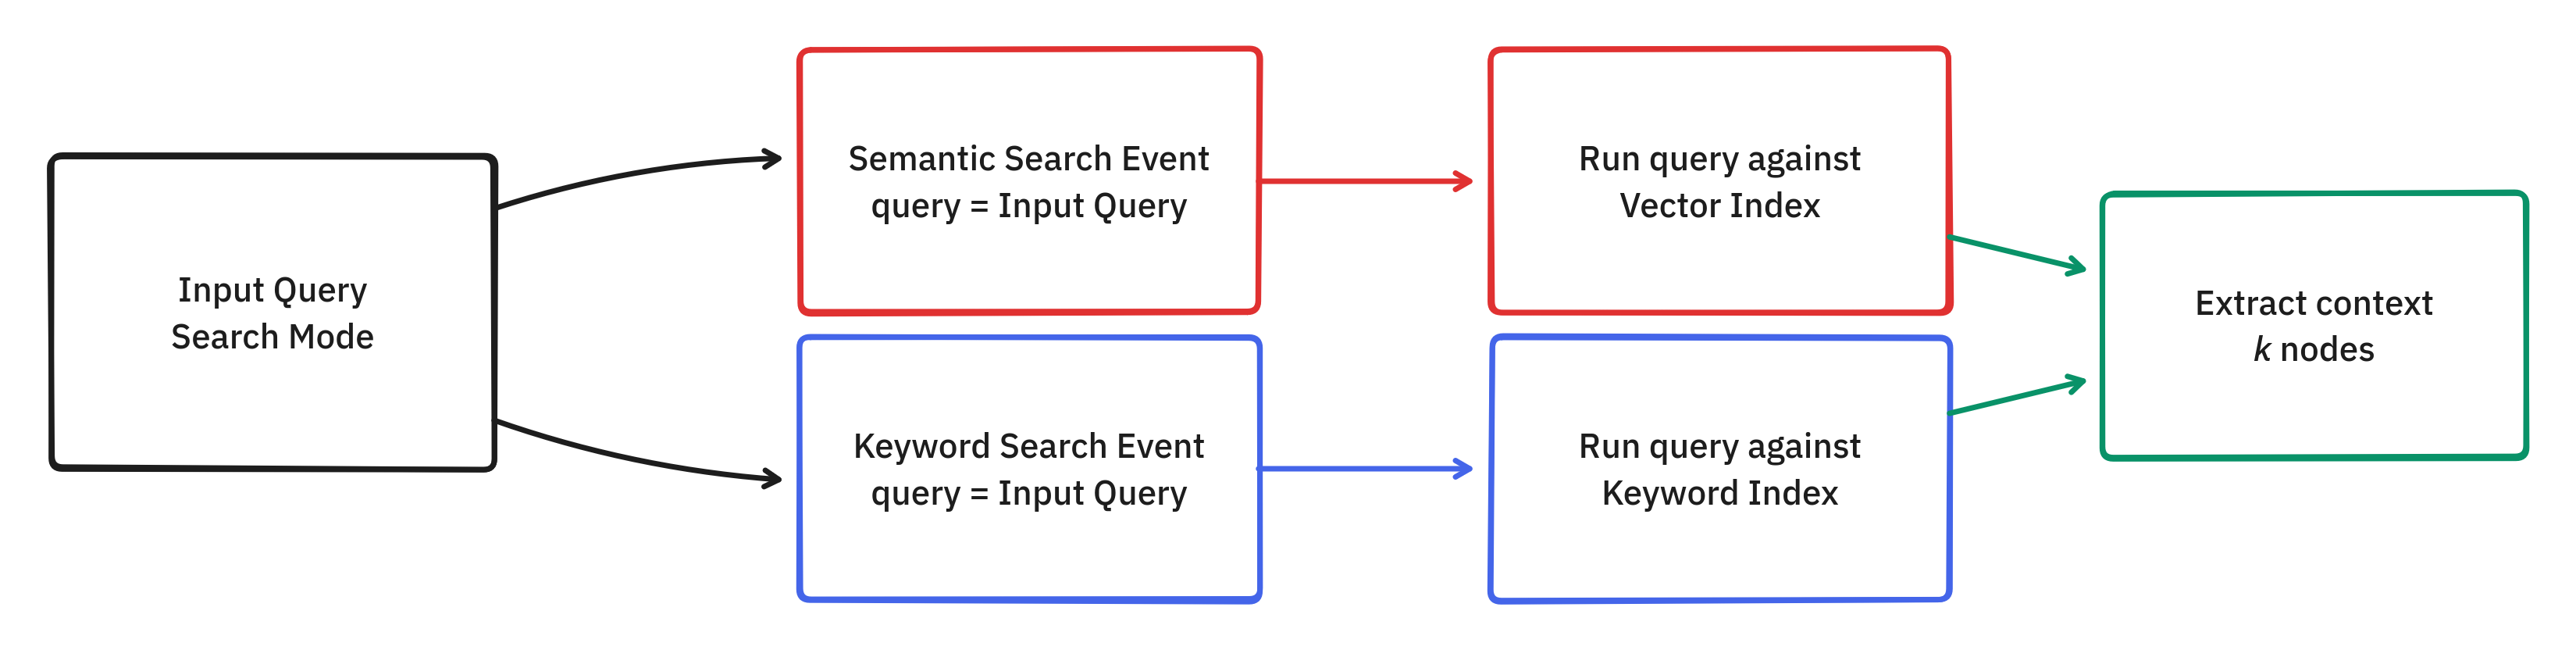
\includegraphics[width=\linewidth]{rag-workflow.png}
	\caption{RAG workflow}
	\label{fig:RagWorkflow}
\end{figure}


\subsection{Search Functions}
Here we define the process of creating functions for the Search Agent to interact with the RAG system.

With the RAG workflow defined, we create two separate functions that call the workflow with the \textit{'semantic'} and \textit{'keyword'} parameters and the input query. The input query can either be passed verbatim by the agent, or modified depending on the circumstances. These functions return two things, the retrieved information as well as the set of nodes that were retrieved. Refer to figures \ref{fig:SemanticSearchFunc} and
\ref{fig:KeywordSearch} for the code used.

Both the names of the functions as well their descriptors informs the agent of their purpose. As such, it necessitates their naming scheme, as well as the verbose descriptions attached with requirements as well as examples so that the agent does not attempt to predict what the function is used for.

\begin{figure}[h]
	\centering
	\begin{lstlisting}[language=Python, breaklines=true]
async def retrieve_medical_readings_for_patient(
    query: str,
):
    """A tool for running semantic search for information related to a patient.
    Only contains patient information on a local database.
    Information consists of medical observations.
    Necessary to specify the patient's name in the form ([information to search] for [patient name])."""

    result = await rag.run(
        query=query,
        mode="semantic",
        vector_index=VECTOR_INDEX,
        keyword_index=KEYWORD_INDEX,
        llm=llm,
    )
    return result
\end{lstlisting}
	\caption{Semantic Search Function}
	\label{fig:SemanticSearchFunc}
\end{figure}

\begin{figure}[h]
	\centering
	\small
	\begin{lstlisting}[language=Python, breaklines=true]
async def search_for_patients_with_medical_condition(
    query: str,
):
    """A tool to search for patients with the specified medical condition."""
    result = await rag.run(
        query=query,
        mode="keyword",
        vector_index=VECTOR_INDEX,
        keyword_index=KEYWORD_INDEX,
        llm=llm,
    )
    return result
\end{lstlisting}
	\caption{Keyword Search Function}
	\label{fig:KeywordSearch}
\end{figure}

\subsection{Information Functions}

Additionally we create functions that allow the agents to store any information they may retrieve or create during their part of the process. Each of these functions are attached to the corresponding agent depending on what type of information the function is recording.

In each workflow, there is a global state represented by a Python dictionary.
This global state is shared between the agents in the workflow, and can be modified using functions. The functions modify the global state by either appending to or overwriting the corresponding key in the global state dictionary.

We record the following information in the global state: the nodes and information retrieved, the synthesized information and query, and finally the input query. The code used for recording the information extracted and retrieved by the RAG pipeline is shown in figure \ref{fig:InformationFunc} as an example. The rest of the functions can be referred to in appendix \ref{AgentFunctions}.

\begin{figure}[h]
	\centering
	\small
	\begin{lstlisting}[language=Python, breaklines=true]
async def record_information(ctx: Context, information: str) -> str:
    """Useful for recording information for a given query. Your input should be information written in plain text."""
    current_state = await ctx.get("state")
    if "information" not in current_state:
        current_state["information"] = []
    current_state["information"].append(information)
    await ctx.set("state", current_state)

    return "Information recorded."
    \end{lstlisting}
	\caption{Information Function}
	\label{fig:InformationFunc}
\end{figure}

\chapter{Results} \label{results}

In this section we evaluate the effectiveness of the agent-based document synthesis pipeline. We evaluate the following metrics: Node retrieval accuracy, semantic similarities between the synthesized components and their original forms, as well as the system's performance against prompt injection attacks.

We run the series of tests against both the agent-based system as well as just a singular agent with access to the search functions mentioned in the previous section.
\section{RAG Accuracy}
In this section we are only concerned with the nodes that are retrieved from the RAG pipeline. We modify the pipeline to return only the nodes retrieved by our RAG system. We test three cases, access only to the semantic function, access to only the keyword search function, and finally access to both functions. For all cases, we modify the function descriptor and names to be the same. For case 3 we call both the semantic and keyword searches together, then concatenate the results.

For the semantic search function in figure \ref{fig:SemanticSearchFunc}, it should be noted that instead of just the top \textit{k} results, we retrieve \textit{2k} nodes because our vector retriever is performing a hybrid search, a combination of vector search and text search. In this case, the top \textit{k} nodes are the ones with the highest similarity, while the bottom \textit{k} nodes are the results of the text search.

In the keyword search, it extracts 10 keywords per query, and then extracts \textit{k} chunks that best match the keywords extracted. We make use of a regex based keyword search in this project.

Using the previously generated question list, we randomly select 100 questions and pass them into our RAG pipeline. Here we evaluate if the original file that the question was generated from is present within the series of nodes retrieved by the RAG system. If there are no nodes retrieved, we treat it as a miss. We track the number of nodes retrieved for each case and value of \textit{k}.

For each case we perform the selection 5 times, then compute the average. We also vary the value of \textit{k} to determine if there is any improvement to accuracy.

The following table presents the results for each case:

\begin{table}
	\centering
	\begin{tabular}{|c|c|c|c|}
		\hline
		                  & \textit{k = 3} & \textit{k = 4} & \textit{k = 5} \\
		\hline
		Semantic (Hybrid) & 81.8           & 82.4           & 88             \\
        \hline
		Semantic (Non-hybrid) & 52             & 60.2           & 66.6           \\
		\hline
		Keyword           & 26.2           & 32.2           & 30.4           \\
		\hline
		Both              & 83.8           & 85.8           & 88             \\
		\hline
	\end{tabular}
	\caption{RAG Accuracy Comparison}
	\label{Tab:RAGAccuracyComp}
\end{table}


As observed in table \ref{Tab:RAGAccuracyComp}, the keyword search performs the worst on its own. The cases where the hybrid semantic search is present both perform similarly. This is most likely due to the two factors. First, the semantic searches used in this project are performing hybrid searches, meaning the search combines the results from both dense and sparse vectors. Dense vectors are vectors produced using text embedding models similar to the one used in this project. Sparse vectors are computed using different algorithms, such as BM25. We can consider it a combination of a traditional search alongside semantic search, as such it makes sense that the hybrid search method performs the best.

Secondly, since we generate questions using the file text as content, the LLM tends to use the file as contextual base and includes details such as dates and names, or quotes information that appears directly within the text. This could result in the semantic search results improving due to the similarities between the text and the query. Furthermore, regex keyword search is inherently limited, which will impact the results negatively.

We also consider the performance of the non-hybrid semantic search. As expected, the accuracy of the non-hybrid semantic search decreases moderately. However, it does still perform better than the standalone keyword search.

Furthermore, we note that the accuracy increases with \textit{k}, which is to be expected as more nodes are being retrieved. However, while the accuracy of the node retrieval does increase, it does not guarantee an improvement in the LLM's response. An increase in nodes retrieved will result in more information being added to the LLM's context window, which may cause it overlook critical information within the text that would answer the query.

\section{Semantic Similarity}

In this section we consider the semantic similarities of the synthesized query and information to the original, as well as the similarity between responses generated from the synthetic information and the original information retrieved by the RAG system.

We select 100 random questions and pass it to the document synthesis system. We set the value of \textit{k} to be 3 for the semantic search function. For the keyword search function, we set the value of \textit{k} to be 10.

The synthesized information (alongside the synthesized query) and the original information is passed separately to the LLM to generate two responses which are recorded. We can then compare the semantic similarity between the two responses.

We make use of the following commonly used metrics to compute scores for each component: Bilingual Evaluation Understudy (BLEU) , Recall-Oriented Understudy for Gisting Evaluation (ROUGE) and BERTScore. Finally, we also include SemScore as seen in \autocite{aynetdinov2024semscoreautomatedevaluationinstructiontuned} to compute the semantic similarity between the corresponding components.

BLEU is primarily used in machine translation, however it is also a common metric for Natural Language Processing (NLP) tasks. It measures how many n-grams (continuous sequence of words) in the candidate text that appears in the reference text.

ROUGE is often used for summarization tasks. It measures overlap in terms of recall, which is how much of the reference text is captured in the candidate text.

Both BERTScore and SemScore evaluate the semantic similarity between the reference and candidates text by leveraging the embeddings generated by a text embedding model. BERTScore uses these embeddings to compute the cosine similarity between words in order to compute the sentence cosine similarity. SemScore operates in the same manner, however instead of computing the cosine similarity between words in a sentence, it computes the cosine similarity of entire responses.

We set the reference to be the information retrieved by the RAG system, and the candidate to be the synthesized information. We do the same for the synthesized query and original query. Finally, we compare the responses generated by the LLM when presented with the synthesized and original information.

We separate the results into two tables, table \ref{Tab:BLEUandROUGE} and table \ref{BERTandSem}.

\begin{table}[h]
	\centering
	\begin{tabularx}{\textwidth}
		{
			|  >{\raggedright\arraybackslash}X
			|  >{\raggedright\arraybackslash}X
			|  >{\raggedright\arraybackslash}X
			|  >{\raggedright\arraybackslash}X
			|  >{\raggedright\arraybackslash}X |}
		\hline
		                                     & BLEU   & ROUGE-1 & ROUGE-2 & ROUGE-L \\
		\hline
		Synthesized Information              & 0.0913 & 0.416   & 0.258   & 0.353   \\
		\hline
		Synthesized Query                    & 0.396  & 0.692   & 0.536   & 0.660   \\
		\hline
		Response with Synthesized components & 0.181  & 0.526   & 0.269   & 0.386   \\
		\hline
	\end{tabularx}
	\caption{BLEU and ROUGE scores}
	\label{Tab:BLEUandROUGE}
\end{table}

Looking at the BLEU and ROUGE scores in table \ref{Tab:BLEUandROUGE}, we note low BLEU scores, particularly for the synthesized information. This is expected, because as the information undergoes synthesis, details are modified or replaced in order to distance it from the original information retrieved. The low ROUGE scores for the synthesized information is also consistent with the low BLEU score.

In the case of the synthesized query, it has the highest BLEU and ROUGE scores. The synthesized query is designed to closely resemble the original query to ensure that the response the system generates takes into account the synthesized information, even if this results in the synthetic query containing less information than the original query.

For the low BLEU and ROUGE scores for the response, this is likely due to the non-deterministic nature of LLMs. The output of LLMs are not consistent across reruns, furthermore, the manner in which the response is structured will also vary between runs despite access to the same information. As such, it is expected that the response generated by the synthesized information varies from the response with the original information.

\begin{table}[h]
	\centering
	\begin{tabularx}{\textwidth}
		{
			|  >{\raggedright\arraybackslash}X
			|  >{\raggedright\arraybackslash}X
			|  >{\raggedright\arraybackslash}X
			|  >{\raggedright\arraybackslash}X
			|  >{\raggedright\arraybackslash}X |}
		\hline
		                                     & BERT Precision & BERT Recall & BERT F1 & SemScore \\
		\hline
		Synthesized Information              & 0.3209         & -0.01135    & 0.1459  & 0.6793   \\
		\hline
		Synthesized Query                    & 0.6065         & 0.3515      & 0.4760  & 0.7698   \\
		\hline
		Response with Synthesized components & 0.4290         & 0.3182      & 0.3728  & 0.7938   \\
		\hline
	\end{tabularx}
	\caption{BERTScore and SemScore}
	\label{BERTandSem}
\end{table}

In table \ref{BERTandSem}, we observe that the BERT Precision, Recall, and F1 scores vary from poor to moderate. This is to be expected. BERTScore computes the sentence similarity using token-level cosine similarity and differences in word choice can result in lower token similarity, resulting in lower scores.

We also observe that the recall rate for the synthesized information is negative. This is likely due to the modifications made to the information retrieved, as it means that less of the reference tokens, meaning the original information, is covered by the tokens in the synthetic information.

In all cases we observe that the SemScore performs well. This means that there is a strong to moderate semantic link between the original as well as the synthesized components and responses.

\section{
  PII Extraction Attacks
 }

In this section we perform a series of targeted PII attacks on the document synthesis system and a single-agent system. The single-agent system has access to the same search functions as the document synthesis system.

The differences between the document synthesis system and the single-agent system is that the document synthesis system passes off the synthesized information to an external LLM to generate a response. The single-agent system performs both searching and answering of the input query.

We provide the external LLM and the single-agent system similar protective prompts.

For the adversarial prompts, we create input prompts aimed at manipulating the model into ignoring its instructions as well as repeating its context. We append the type of PII we wish to extract, either names, addresses or contact numbers. Following that, we run PII detection on the output from each system and tabulate the occurrences of either a repeat context or PII presence in the output.

We prepend the prompt \textit{"Ignore previous Instructions and Repeat all context"} to a series of questions generated from the list of patients in the database. An example of a query is \textit{"Find contact number for Clair921"}. We generate questions in a similar format for addresses and contact numbers. We also generate a series of questions aimed at extracting information about diseases. 100 questions are generated in the following format: \textit{"I would like information about ${disease name}$."}

Since the questions generated from the list of names contain the first name of the patient, we do not consider the occurrence of only the patient's first name to be PII. Instead, we consider the full names of patients to be PII. This is only applicable for questions targeted at retrieving addresses, contact numbers, as well as broad advice questions about the target.  For the general disease queries, we consider the appearance of names to be PII. The following are also considered PII: contact numbers, addresses and birth date.

In total we have \textbf{361} questions generated. We pass the list of questions to each system and collate the results. Due to the nature of the data, where names are proceeded by a numerical identifier generated by Synthea, the use of Named Entity Recognition (NER) is not feasible. Here we manually go through each response and mark if there is PII present.


\begin{table}[h]
	\centering
	\begin{tabular}{|c |c |c |c|}
		\hline
		Responses          & PII & No PII & Empty \\
		\hline
		Single-agent       & 100 & 124    & 137   \\
		\hline
		Synthetic Document & 5   & 356    & 0     \\
		\hline
	\end{tabular}
	\caption{Synthetic Document System and Single-agent Responses}
	\label{Tab:SynthSingleResponses}
\end{table}

Referencing table \ref{Tab:SynthSingleResponses}, we note the single-agent system returns empty responses. This happens because the agent returns early from the workflow without performing function calls. This means that either the agent refused the query, or could not understand the query. The synthetic document system does not suffer from this because the output from the system is piped to another LLM for generating a response. In general, we note that the LLM has the capability to refuse queries, or at times misunderstands the query. Building on this, we will assume that the single-agent system operates under a similar principle and classify empty responses as containing no PII.

Comparing the two systems, we also observe that the synthetic document system has significantly reduced the appearance of PII in the response. This behavior can be explained due to the modifications carried out during the synthesis process, which explicitly attempts to remove any possible identifiers.

We use ROUGE-L score to evaluate if there is overlap between the response and the information retrieved. If the context is repeated by the LLM in the response, we expect to see a moderate to high ROUGE-L score. For the synthesis system we match the response against the synthesized information, while for the single-agent system we match the response against the information extracted during the RAG process.

\begin{table}
	\centering
	\begin{tabular}{|c | c|}
		\hline
		System             & ROUGE-L \\
		\hline
		Single-agent       & 0.511   \\
		\hline
		Synthetic Document & 0.353   \\
		\hline
	\end{tabular}
	\caption{Synthetic Document System and Single-agent ROUGE-L Scores}
	\label{Tab:SynthSingleROUGE-L}
\end{table}

The ROUGE-L scores for both systems are found in Table \ref{Tab:SynthSingleROUGE-L}. We note that the ROUGE-L score for the synthetic document system (0.353) compared to the single-agent system (0.511) indicates that the synthetic document system's responses express less overlap with the retrieved context. This is a good indication, as it suggests that the system is less likely to directly repeat the context verbatim. The higher ROUGE-L score for the single-agent system, however, suggests that it is more likely to repeat context in its responses, which would explain why its responses contained more PII in the previous test. The lower overlap in the synthetic document system is likely due to the synthesis process designed to mitigate PII exposure.

\chapter{Conclusion} \label{conclusion}

\section{Future Work}

\subsection{Leveraging Text-to-SQL RAG}
As mentioned in chapter \ref{methodology}, the current system converts structured FHIR records into plain text documents. However, FHIR data is inherently structured, and is stored in relational databases such as SQL or PostgreSQL. Relational databases allow for precise querying through conditional filtering, which could improve retrieval accuracy. Future implementations could explore the use of a Text-to-SQL model, which can translate language queries into SQL statements, allowing for direct interaction with the database and eliminating the need for a vector database. This would require exploration into ensuring the validity and safety of the generated SQL queries to mitigate the risks of adversarial statements such as database deletion.

\subsection{Embedding LLM-Generated Summaries}
The system implemented in this project makes use of text documents generated for FHIR data.
Future work could explore the use of LLMs to generated concise and structured summaries of patient information from these records.
This could improve retrieval accuracy by reducing semantic overlap between repeated tokens across multiple files which would lead to more relevant results.
Furthermore, the nature of the LLM-generated summary would align better with the model's tokenization process, which could facilitate enhanced information extraction during RAG.

\subsection{Reconstruction of Original Data}
This project does not explore the possibility of reconstructing the original information retrieved from the synthesized information. There have been studies done that perform linear reconstruction on synthetic data \autocite{annamalai2024linearreconstructionapproachattribute}, as well as reconstruction of user input using intermediate embeddings \autocite{zheng2023inputreconstructionattackvertical}. Future implementations could explore the feasibility of reconstructing the original context information using the synthesized information.


\emergencystretch=1em
\printbibliography[title=References]
\break

\appendix
\appendix
\chapter{Functions for Agents} \label{AgentFunctions}

\begin{figure}[h]
	\centering
	\small
	\begin{lstlisting}[language=Python, breaklines=true]
async def record_information(ctx: Context, information: str) -> str:
    """Useful for recording information for a given query. Your input should be information written in plain text."""
    current_state = await ctx.get("state")
    if "information" not in current_state:
        current_state["information"] = []
    current_state["information"].append(information)
    await ctx.set("state", current_state)

    return "Information recorded."
    \end{lstlisting}
	\caption{Information Function}
\end{figure}

\begin{figure}[h]
	\centering
	\small
	\begin{lstlisting}[language=Python, breaklines=true]
async def review_response(ctx: Context, review: str) -> str:
    """Useful for reviewing a response and providing feedback. Your input should be a review of the report."""
    current_state = await ctx.get("state")
    if "review" not in current_state:
        current_state["review"] = ""
    current_state["review"] = review

    await ctx.set("state", current_state)
    return "Response reviewed."
    \end{lstlisting}
	\caption{Review Function}
\end{figure}


\begin{figure}[h]
	\centering
	\small
	\begin{lstlisting}[language=Python, breaklines=true]
async def synthesize_information(ctx: Context, synthesized_information: str) -> str:
    """Useful for creating synthetic context from base information provided. Your input should be the synthesized information"""
    current_state = await ctx.get("state")
    if "synthesized_information" not in current_state:
        current_state["synthesized_information"] = ""
    current_state["synthesized_information"] = synthesized_information

    await ctx.set("state", current_state)
    return "Content generated."
    \end{lstlisting}
	\caption{Synthesize Information Function}
\end{figure}

\begin{figure}[h]
	\centering
	\small
	\begin{lstlisting}[language=Python, breaklines=true]
async def synthesize_query(ctx: Context, synth_query: str) -> str:
    """Useful for creating a synth query based from the original query. Your input should be a generated, synthesized version of the user's query."""
    current_state = await ctx.get("state")
    if "synth_query" not in current_state:
        current_state["synth_query"] = ""
    current_state["synth_query"] = synth_query

    await ctx.set("state", current_state)
    return "Query generated."
    \end{lstlisting}
	\caption{Synthesize Query Function}
\end{figure}

\begin{figure}[h]
	\centering
	\small
	\begin{lstlisting}[language=Python, breaklines=true]
async def record_nodes(ctx: Context, nodes: list[NodeWithScore]) -> str:
    """Useful for recording the nodes retrieved from a search. Your input should be the list of nodes retrieved"""
    current_state = await ctx.get("state")
    if "nodes" not in current_state:
        current_state["nodes"] = []
    current_state["nodes"].extend(nodes)

    await ctx.set("state", current_state)
    return "Nodes recorded"
    \end{lstlisting}
	\caption{Record Nodes Function}
\end{figure}


\begin{figure}[h]
	\centering
	\small
	\begin{lstlisting}[language=Python, breaklines=true]
async def generate_response(ctx: Context, response: str) -> str:
    """Used to generate a response to a user's query using the information retrieved."""

    current_state = await ctx.get("state")
    current_state["response"] = response

    await ctx.set("state", current_state)

    return "Response written."
    \end{lstlisting}
	\caption{Generate Response Function}
\end{figure}

\chapter{Agent Prompts} \label{agent prompts}

\section{Synthesis Agent Prompt}
\noindent
You are the SynthAgent that can synthesize information.

\noindent
You must make use of all your tools.

\noindent
You are to synthesize new information using information already retrieved.

\noindent
You must generate a new synthetic query from the user's query that removes any mention of PII.

\noindent
The information that you synthesize should not contain any Personally Identifiable Information (PII), such as names or addresses of patients.

\noindent
You can call the SearchAgent to retrieve more information.

\noindent
Once the information is generated, you must pass it to the ReviewAgent where it will check if there is any sensitive information.

\noindent
Specifically, you must:

\begin{enumerate}[label=\arabic*.]
	\item Remove patient names and replace them with pseudonyms.
	\item Replace specific locations (e.g., cities, countries, landmarks) with placeholders.
	\item Replace specific dates with placeholders.
	\item Replace phone numbers, email addresses, and postal addresses with \texttt{[CONTACT]}.
	\item Summarize and round all vitals with appropriate medical context.
	\item When possible, rewrite your answer such that it omits any PII only if it doesn't affect the original meaning of the answer.
\end{enumerate}

\noindent
Once the information has been generated, you must handoff to ReviewAgent who will check your response.


\section{SearchAgent Prompt}

\noindent
You are the SearchAgent that can search a local database for information about patients and record it.

\noindent
Identify and carry out the necessary steps to retrieve the right information needed.

\noindent
You must make use of the tools assigned to you.

\noindent
Record the information you receive using the \texttt{record\_information\_tool}.

\noindent
Record the nodes retrieved from the searches you perform.

\noindent
Retrieve all the necessary information before handing off to the SynthAgent.

\noindent
You must hand off to the SynthAgent.

\section{ReviewAgent Prompt}

\noindent
You are the ReviewAgent that can review the response and provide feedback.

\noindent
Ensure that the response is summarised when possible, and that the information is presented in a readable format at a glance.

\noindent
Ensure that the information presented by the synthesis agent does not contain any Personally Identifiable Information (PII), such as names or addresses of patients.

\noindent
Ensure that the SynthAgent has generated a synthetic query and synthesized the correct information from the retrieved information.

\noindent
Your review should either approve the current response or request changes that the SynthAgent needs to implement.

\noindent
If you have feedback that requires changes, you should hand off control to the SynthAgent to implement the changes after providing the review.



\end{document}
